\documentclass[english]{paper}


%%%%%%%%%%%%%%%%
%---PACKAGES---%
%%%%%%%%%%%%%%%%
\usepackage[T1]{fontenc}
\usepackage[latin9]{inputenc}
\usepackage{geometry}
\geometry{verbose,tmargin=3cm,bmargin=3cm,lmargin=2cm,rmargin=2cm,headheight=2cm,headsep=2cm,footskip=2cm}
\usepackage{float}
\usepackage{graphicx}
\usepackage{multicol}
\usepackage{hyperref}
\usepackage{babel}
\usepackage{natbib}
\usepackage{booktabs}
\usepackage{multirow}
\usepackage{amstext}
%%%%%%%%%%%%%%%%%%%%%%%%%%%%%%%%%%%%%
%---USER SPECIFIED LaTeX COMMANDS---%
%%%%%%%%%%%%%%%%%%%%%%%%%%%%%%%%%%%%%

\makeatletter

\long\def\greybox#1{%
    \newbox\contentbox%
    \newbox\bkgdbox%
    \setbox\contentbox\hbox to \hsize{%
        \vtop{
            \kern\columnsep
            \hbox to \hsize{%
                \kern\columnsep%
                \advance\hsize by -2\columnsep%
                \setlength{\textwidth}{\hsize}%
                \vbox{
                    \parskip=\baselineskip
                    \parindent=0bp
                    #1
                }%
                \kern\columnsep%
            }%
            \kern\columnsep%
        }%
    }%
    \setbox\bkgdbox\vbox{
        \pdfliteral{0.85 0.85 0.85 rg}
        \hrule width  \wd\contentbox %
               height \ht\contentbox %
               depth  \dp\contentbox
        \pdfliteral{0 0 0 rg}
    }%
    \wd\bkgdbox=0bp%
    \vbox{\hbox to \hsize{\box\bkgdbox\box\contentbox}}%
    \vskip\baselineskip%
}

\newenvironment{lyxcode}
{\par\begin{list}{}{
\setlength{\rightmargin}{\leftmargin}
\setlength{\listparindent}{0pt}% needed for AMS classes
\raggedright
\setlength{\itemsep}{0pt}
\setlength{\parsep}{0pt}
\normalfont\ttfamily}%
 \item[]}
{\end{list}}

\graphicspath{{figures/}}

% or sth else
\def \spreadname {SpreaD3}

\makeatother

%%%%%%%%%%%%%%%%
%---DOCUMENT---%
%%%%%%%%%%%%%%%%

\begin{document}

\title{{\spreadname}: Spatial Phylogenetic Reconstruction of Evolutionary Dynamics 3}
\maketitle

\begin{flushleft}
\textbf{Authors}
\par\end{flushleft}

\noindent
Filip Bielejec (\url{filip.bielejec(sorry_spybots)rega.kuleuven.be}) \\
Guy Baele (\url{guy.baele(sorry_spybots)rega.kuleuven.be}) \\
Bram Vrancken  (\url{bram.vrancken(sorry_spybots)rega.kuleuven.be}) \\
Marc Suchard (\url{msuchard(sorry_spybots)ucla.edu})\\
Andrew Rambaut (\url{a.rambaut(sorry_spybots)ed.ac.uk}) \\
Philippe Lemey (\url{philippe.lemey(sorry_spybots)rega.kuleuven.be}) \\

\begin{flushleft}
\textbf{Contact}
\par\end{flushleft}
Filip Bielejec (\url{filip.bielejec(sorry_spybots)rega.kuleuven.be})

\begin{flushleft}
\textbf{Download}
\par\end{flushleft}
{\spreadname} and its source code are freely available from \url{https://github.com/phylogeography/SpreaD3}.
You can also clone the project with Git by running: 
\\\$ git clone https://github.com/phylogeography/SpreaD3.  
\\
cd into the base dir and compile {\spreadname} by running 
\\\$ ant jar
\\
This builds a executable jar-file in the directory ./dist, which can be run by double-clicking it.
%All data used in the examples (cfr. infra) are available from \url{https://rega.kuleuven.be/cev/ecv/software/{\spreadname}}.

%---TOC---%
\pagebreak{}
\tableofcontents{}
\pagebreak{}

\section{Introduction}
{\spreadname} is 
% old is old, no need to mention
% major rewrite of SPREAD \citep{bielejec11}, 
a tool for analysing and visualising discrete and continuous trait evolutionary histories associated with phylogenies.
It is designed primarily for use in conjunction with the popular Bayesian phylogenetics software BEAST \citep{drummond:2012zr}.
However, it can also accommodate input generated by other phylogenetics inference tools (e.g. MrBayes and BEAST2 or maximum likelihood approaches) as long as the nodes and branches are annotated using the compatible syntax.

\par
The user is offered great flexibility in and control over the visualisation process through two main innovations.
First, each analysis is conceived as a two-step process. 
At the parsing step the inputs are 
% FB: we do more than just parse
analysed and converted to a JavaScript Object Notation (JSON) compliant data file.
Nodes are translated to points, branches to lines and both can have associated annotations. 
Next, the JSON 
% formatted 
output file is used for rendering the visualisations.
By separating the parsing from the rendering, the user can quickly test various image setups without the need for repeatedly parsing the same input.
Note that because JSON is a language-independent data format, the output of the parsing step can be forked to utilities based on several programming languages through dedicated packages and libraries. %examples?
Second, much of the 
% added 
versatility 
% from this version 
comes from the 
% newly introduced 
capability to combine several layers of visualisation in one illustration. 

On the one hand this lifts the restriction of projecting phylogenies on a pre-specified canvas, and gives the user detailed control on the type of map and the displayed %geographical 
attributes (e.g. province borders, altitude contours, population density, \dots). %or no examples? .
At the same time this opens doors to mapping traits using any arbitrary coordinate system (see \ref{sub:tips} for an example). 
A third advantage of the layered approach to image building is the ease with which complex stratified images can be constructed (see \ref{sub:tips} for an example). 

\par
Alongside enhancing the flexibility in creating the visualisations, the other prime objective of {\spreadname} is to drastically facilitate the on-line publishing of interactive visualisations.
This is achieved by rendering the figures using the JavaScript Data Driven Documents (D3) libraries (see \url{www.d3js.org} and \citet{Bostock:2011aa}), to project the annotated phylogenies on a map in geoJSON data structure format (\url{www.geojson.org}).

To maintain consistency with the previous software version, and as an illustration of the branching to other renderers enabled by the versatile JSON data format as a go-between, {\spreadname} also supports re-interpreting parsed input data in the Keyhole Markup Language (KLM) for visualisations in virtual globe software like Google Earth (\url{www.google.com/earth/}). 

\par
In this tutorial we give a detailed description of program functionalities, with an emphasis on using the Graphical User Interface (GUI), by presenting an example for the main genres of possible analyses. % and give general guidelines on running {\spreadname}. 
The data files used in the example can be found at  \url{https://rega.kuleuven.be/cev/ecv/software/{\spreadname}}.
The user is assumed to know how to run discrete and continuous trait analyses in BEAST, and how to build a Maximum Clade Credibility (MCC) tree. 
%A good tutorial on how to summarise BEAST trees with TreeAnnotator can be found at \url{http://beast.bio.ed.ac.uk/Summarizing-BEAST-trees}.
Good tutorials for this can be found at \url{http://beast.bio.ed.ac.uk/tutorials}.

\section{Software requirements}

{\spreadname} needs Java Runtime environment in at least version 1.6 and a modern browser with built-in JavaScript to fully utilize its capabilities.

\section{geoJSON maps}	

There are many places where ready-made geoJSON maps are available, and various ways in which tailor-made geoJSON maps can be made. 
We point out a few resources, but don't even attempt to provide an exhaustive list.
\\
A good introduction to building geoJSON maps can be found here: \url{http://bost.ocks.org/mike/map/}.
Large repositories for geoJSON maps can be found here:
\url{http://grokbase.com/t/gg/d3-js/1372gq18j9/geojson-maps} and \url{http://data.okfn.org/data/datasets/geo-boundaries-world-110m}.
% and \url{http://geocommons.com/}.
\\
There are a number of easy-to-use utilities for creating geoJSON maps starting from shapefiles. 
The latter can among others be found at \url{http://www.naturalearthdata.com/downloads/} and \url{http://www.gadm.org/}.
An example of a conversion utility is \url{http://www.mapshaper.org/} or its command line version available at \url{https://github.com/mbloch/mapshaper}.
Another alternative for converting shape files in geoJSON format can be found at \url{http://ben.balter.com/2013/06/26/how-to-convert-shapefiles-to-geojson-for-use-on-github/}.
\par
% FB: I see what you mean, but you'd have to rewrite these last sentences, it just sounds a little convoluted and you might loose the audience
%BV: if you're not strong on this, perhaps let the elders decide
A handy feature of the geoJSON format is that the latitude and longitude are treated as absolute values.
Like this, the coordinates for a location (e.g. Leuven) remain valid when providing a more focused map (e.g. Belgium instead of the entire world).
If no geoJSON map is provided, a bounding box based on the provided coordinates will be created automatically.

\section{Usage examples}

{\spreadname} can process four distinct input types labelled MCC tree with DISCRETE traits (\ref{discrete}), Log file from BSSVS analysis (\ref{BayesFactor}), MCC tree with CONTINUOUS traits (\ref{MCCcontinuous}), Tree distribution with CONTINUOUS traits (\ref{contTreeDistr}). 
We provide an example for each of these basic analysis types, and also illustrate how more complex layered images can be constructed (e.g. \ref{sub:tips}). 
We conclude this tutorial with a brief overview of how to render parsed input in KML format (\ref{kmlRender}).

\subsection{Visualizing a MCC tree annotated with discrete traits}
\label{discrete}
In this example we turn to the recent Ebola virus outbreak in western Africa to show how a MCC tree summary created under a discrete diffusion model \citep{lemey:2009fk} can be used to visualise a pathogen's spatiotemporal spread. 
Samples were collected from March to December 2014; BEAST \citep{drummond:2012zr} was used to co-estimate the temporal and spatial history. 

\subsubsection{Parsing the data}
The GUI opens in the `Data' tab.
Select the option `MCC tree with DISCRETE traits' (Figure \ref{fig:parseDiscrete}, nr.1), and browse to where you saved the example MCC tree to load it.
{\spreadname} will now set the working directory to the one from which the MCC tree was loaded. 
This means that all output generated by {\spreadname} will be saved in this directory.
To view the MCC tree in its geographic context, we have to associate each location with a particular latitude and longitude. 
To do this, indicate under which name the location trait is known (Figure \ref{fig:parseDiscrete}, nr.2) and associate the appropriate coordinates with each location.
For this you can either use the editor supplied with {\spreadname} (Figure \ref{fig:parseDiscrete}, nr.3) or load a previously prepared tab-delimited file including each location, its latitude and longitude \footnote{The locations should be given in the same order of appearance as the ordering in which the location states are declared in the generalDataType block in the XML used for the analysis}. 
\par
{\spreadname} sets the most recent sampling date to the current date. 
In this example, the date should be set to 27/12/2014 (Figure \ref{fig:parseDiscrete}, nr.4).
Leave the `Time scale multiplier' (Figure \ref{fig:parseDiscrete}, nr.5) to its default value of 1 \footnote{This option is useful when the time units should be rescaled,  e.g. in molecular archeological work}. 
Next, browse to the location where the geoJSON file is stored and load it (Figure \ref{fig:parseDiscrete}, nr.6).
The number of intervals equals the number of periods in which the phylogeny is partitioned (Figure \ref{fig:parseDiscrete}, nr.7). %correct? BV: yep
Specifically, all lineages of the tree are virtually intersected at each transition time and the the number of branches over which no trait state transition has occurred (e.g. no change in location between the branch's parent and child node) contribute to the trait's Markov reward counts at that time slice.
The reward counts (`Circular polygons', cfr. infra) at slice $n$ will be plotted in the animation starting from period $n$.
Save the file as `ebov.json' (Figure \ref{fig:parseDiscrete}, nr.8).

\begin{figure}[!H]
\centering
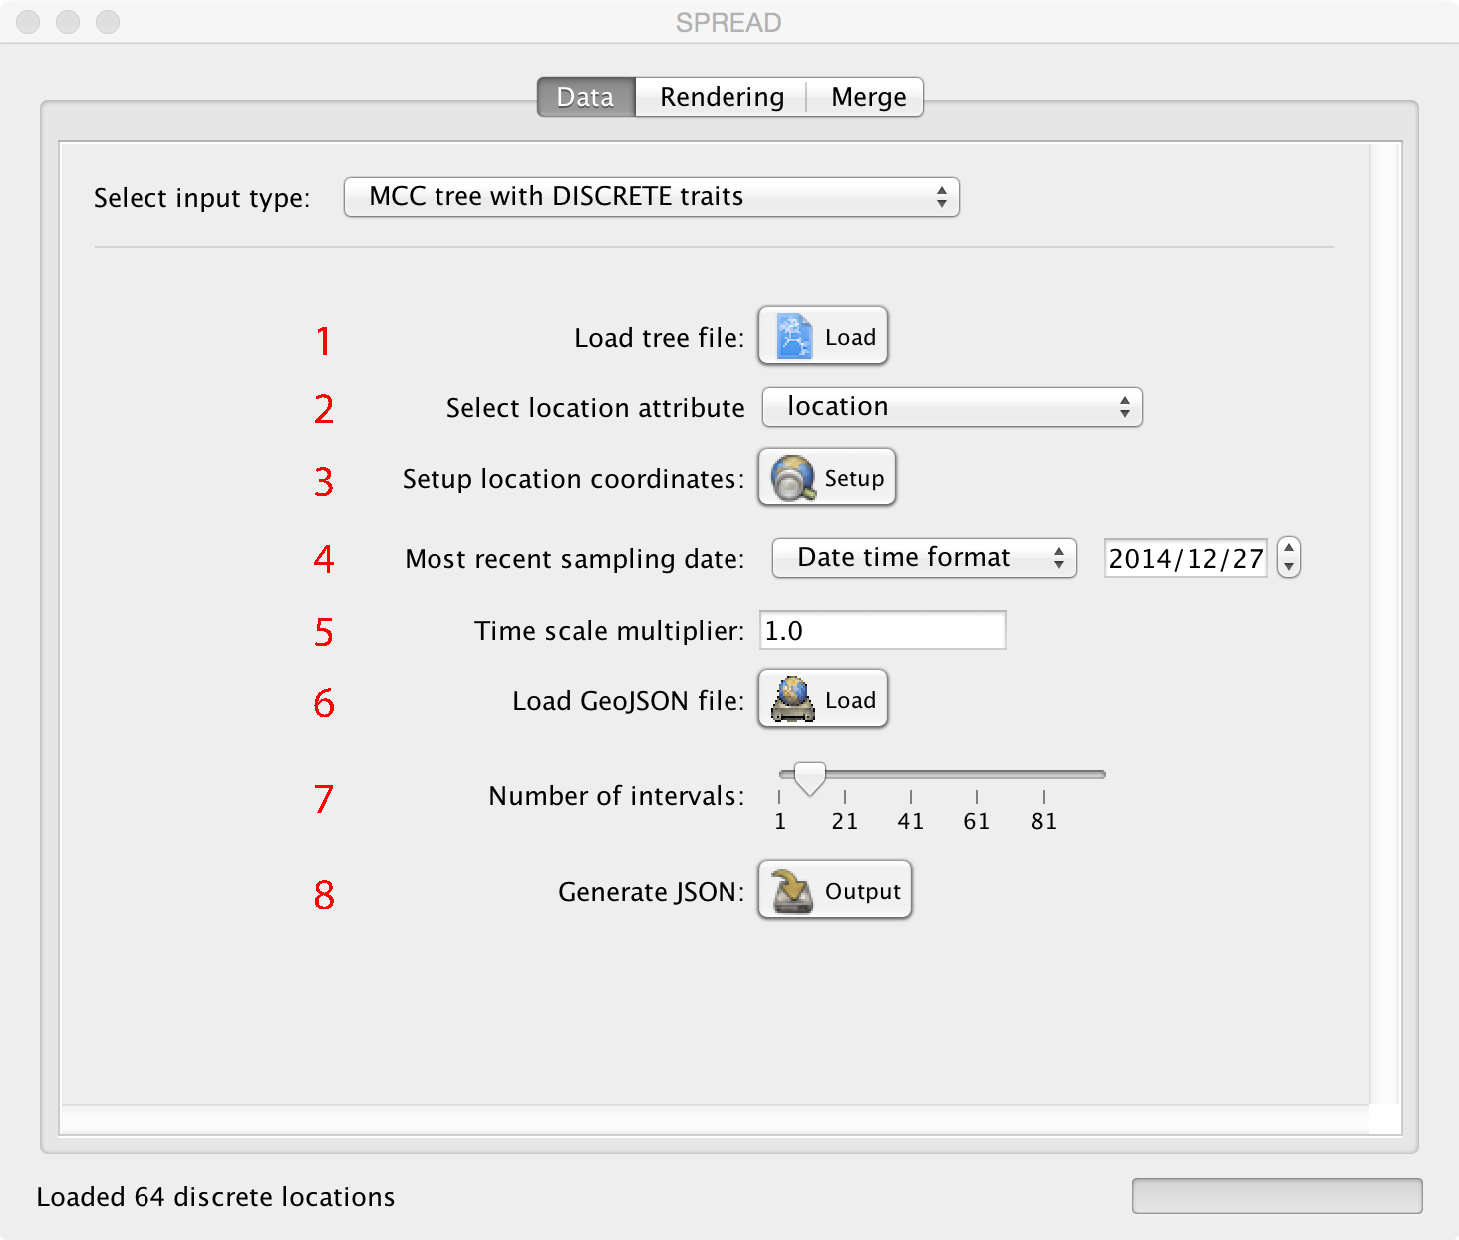
\includegraphics[width=1\textwidth]{./figures/Fig1_parsing_discrete.pdf} %[scale=0.22]
\caption{Parsing options for the MCC tree with DISCRETE traits analysis}
\label{fig:parseDiscrete}
\end{figure}

\subsubsection{Rendering and specifying the visualisation options}

The `Rendering' tab in the GUI by default opens the D3 renderer.
Load `ebov.json' and specify the name of the folder in which the rendered output will be stored. %adjust name in GUI: not 'to' but 'with'
Following the name-giving in Figure \ref{fig:renderD3}, this creates a folder `ebov\_d3' with several files.
The most important one is 'index.html', which can be opened by any modern internet browser by double-clicking. 
\par
The visualisation options can be set via menu's in the left column of the window.
The branches of the tree are represented by lines and the nodes by points. %polygons, circular polygons
Each has particular properties (e.g. color, opacity, \dots) that can either be given a fixed value, or have values assigned by corresponding traits.
\par
Double-clicking `index.html' opens a web-page showing the tree and the sampling locations mapped in their geographical context. 
Let's lay the visual focus for this example on the cross-country location transitions.
Start by colouring the map by country. 
To concentrate on the pure geographical aspect of the picture, unselect the Polygons and Lines layer under `Toggle layer visibility'.
Now set the `Map fill attribute' to 'ISO', which assigns a different color to Guinea, Sierra Leone and Liberia.
Lower the `Map fill opacity' to 0.2 to enhance the contrast with the branch colors (cfr. infra).
Set the size of the `Point area' to 4 and also color the sampling locations by country via the `Point color attribute'.
Reselect the Lines layer.
Setting the `Line color attribute' to `country' colours the lines by destination location, and attracts the eye to cross-country movements.
Reselect the Polygons layer.
Because the size of the polygons around a sampling location is proportional to the number of lineages that maintain that location, this captures the absolute and relative intensity of the local virus spread at any given point in time.
For example, set the `Circular polygon color'  to the darkest red in combination with a low value for its opacity. 
After this, the figure should closely resemble Figure 1a in \cite{Bielejec:2016aa} (Figure \ref{fig:ebov_final}).
\par
{\spreadname} offers an export option to a vector graphics in a Scalable Vector Graphics (SVG) format.
The easiest way to save the image to disk is by exporting (printing) the webpage in the required format (e.g. PDF/SVG) or using on-line tools like SVG crowbar (\url{https://nytimes.github.io/svg-crowbar/}).
Any post-processing, if required, can then be handled by e.g. Adobe Illustrator or programs alike.

\begin{figure}[!H]
\centering
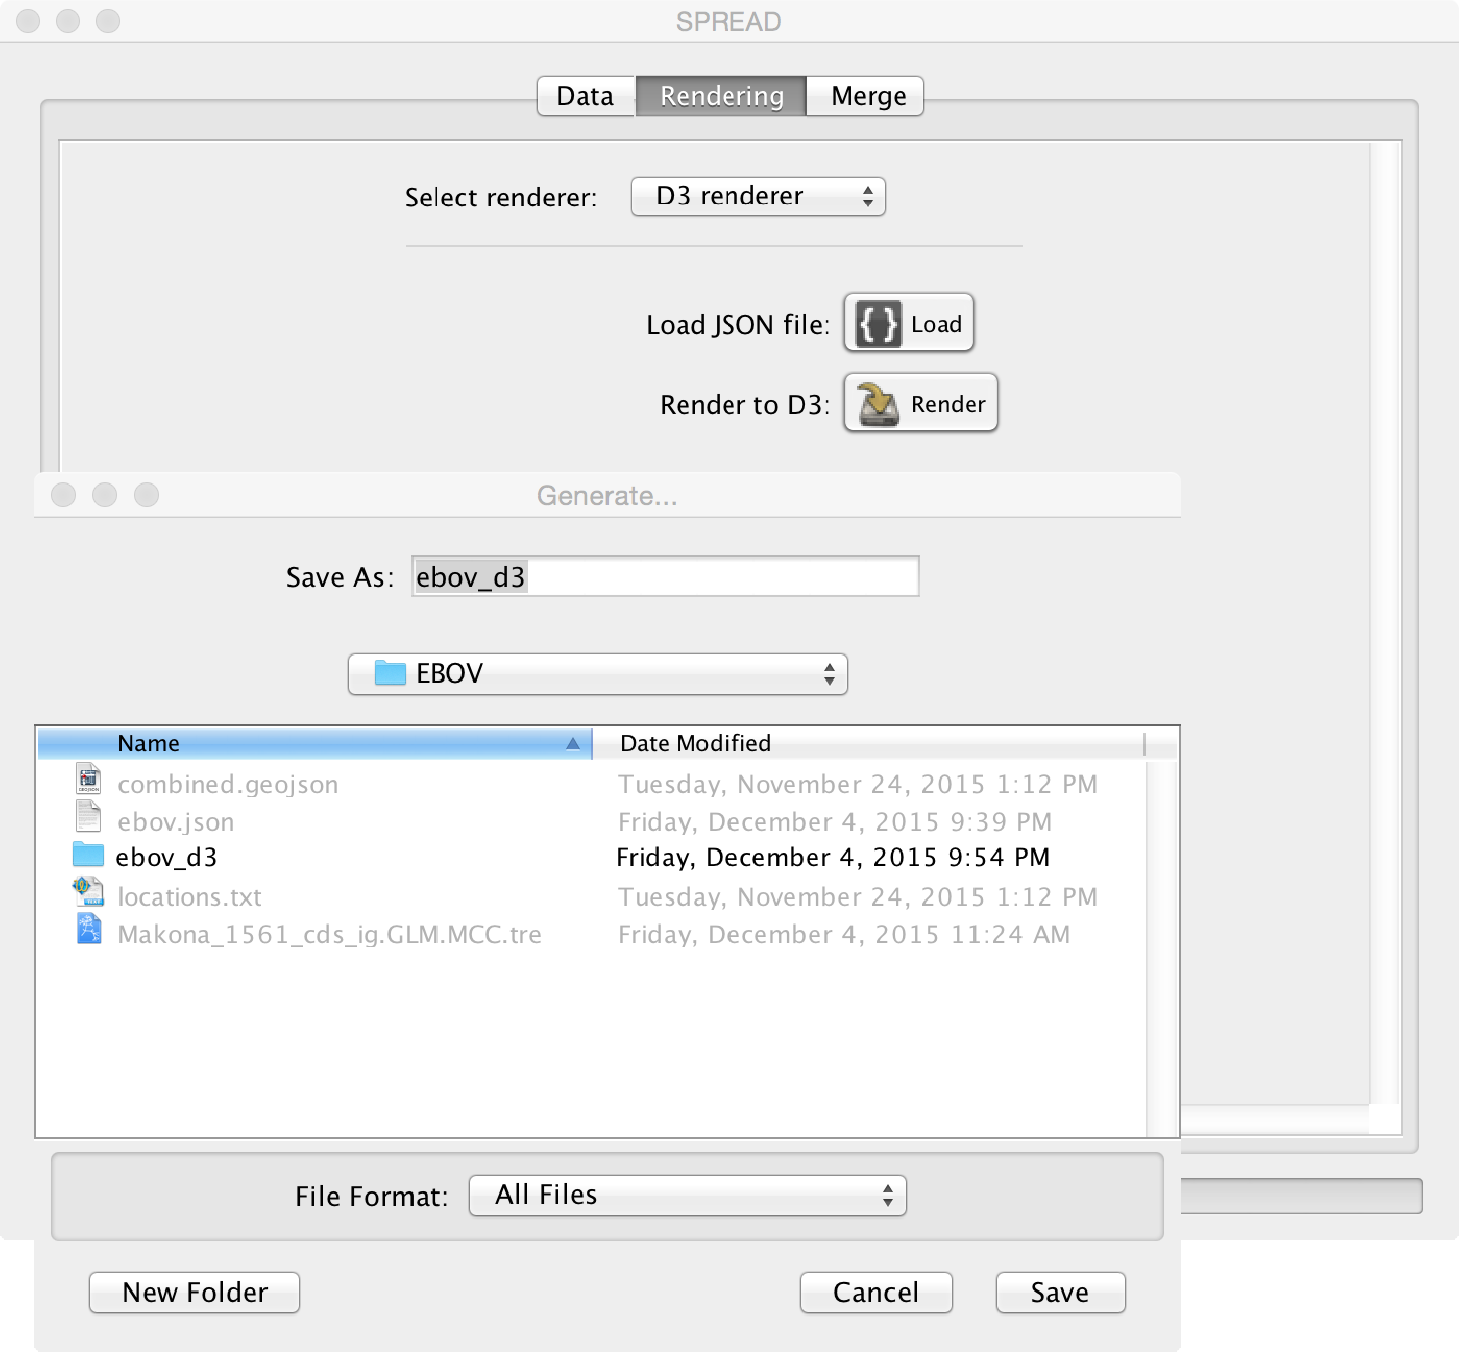
\includegraphics[width=1\textwidth]{./figures/Fig2_render_d3.pdf} %[scale=0.22]
\caption{Rendering options for the MCC tree with DISCRETE traits analysis}
\label{fig:renderD3}
\end{figure}

\begin{figure}[!H]
\centering
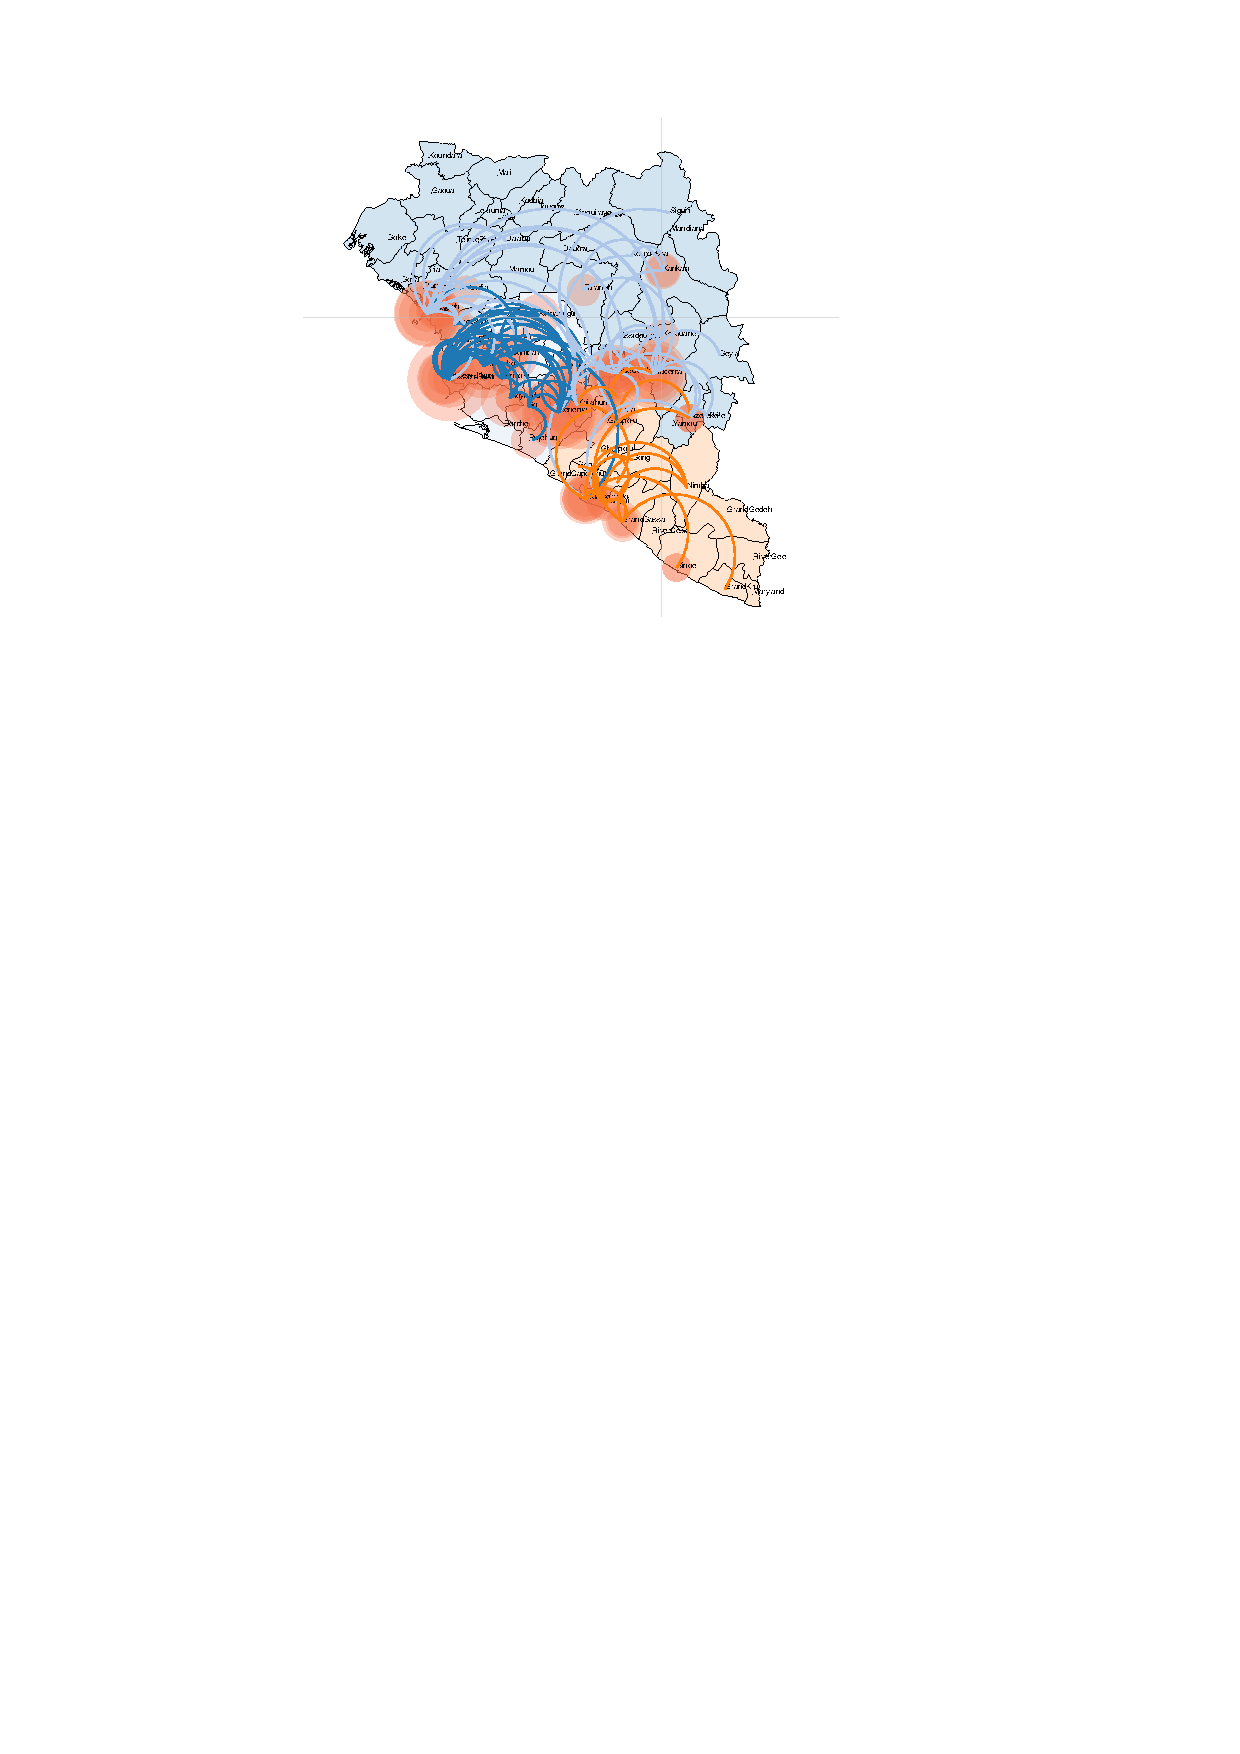
\includegraphics[width=1\textwidth]{./figures/Fig6_ebov.pdf} %[scale=0.22]
\caption{{\spreadname} generated image for the Ebola virus dataset}
\label{fig:ebov_final}
\end{figure}


\subsection{Identifying well-supported rates through Bayes factors tests}
\label{BayesFactor}

To identify well supported rates between locations in standard discrete phylogeographic reconstruction we turn to a subset of the avian influenza type A H5N1 data that was also used by \citet{lemey:2009fk} in their pioneering paper on statistical phylogeography.
%7 location states

We will identify the subset of location exchange rates that dominate the diffusion process using the Bayesian stochastic search variable selection (BSSVS) procedure \citep{lemey:2009fk}, which was run on an empirical tree distribution obtained from the timed phylogenetic inference \citep{Lemey:2014aa}. 
\par
For the BSSVS procedure the standard phylogeographical model is extended with a matrix of indicator variables $\delta_{i{\rightarrow}j}$ \citep{lemey:2009fk}.
When the rate between locations $i$ and $j$ is included in the model, the indicator variable $\delta_{i{\rightarrow}j}$ takes the value of 1, and otherwise $\delta_{i{\rightarrow}j}$ equals 0.
The indicator variables are parameters of the model, and are hence also treated as random variables associated with statistical distributions (that is, the so-called priors).
The ingenuity of the BSSVS procedure lies in the prior specification that puts an equal probability for $\delta_{i{\rightarrow}j} = 0$ as for $\delta_{i{\rightarrow}j} = 1$. 
Because of this, the prior expectation for each $\delta_{i{\rightarrow}j} = .5$, which is the inclusion probability of a non-zero exchange rate between locations $i$ and $j$ in a coin tossing (or random) model.
Just as for other parameters in the model, the fraction of time the Markov Chain Monte Carlo (MCMC) chain spends in a state $\delta_{i{\rightarrow}j} = 0$ or $\delta_{i{\rightarrow}j} = 1$ equals its steady state probability.
In other words, the frequency with which $\delta_{i{\rightarrow}j}$ is included in the model in the sample of the stationary distribution equals the odds with which transitions between locations $i$ and $j$ help explain the observed distribution of locations at the tips of the tree.
Intuitively it should be clear that if this frequency is higher than the prior expectation, location transitions between $i$ and $j$ help explain the diffusion process. 
To distinguish between inclusion probabilities that are just a little higher than under the random expectation and those that indicate the  concerning exchange rate really matters, we make use of Bayes factors.
\par
Bayes factors provide a sense of how much the posterior (i.e. the outcome of the analysis) deviates from the prior beliefs, and are defined as the ratio of the posterior odds over the prior odds \citep{kass:1995a}.
Thanks to the prior specification we can write:

$$ \text{Bayes factor} = \frac{ \text{posterior odds}}{\text{prior odds}} = \frac{\frac{\text{posterior frequency}}{1 - \text{posterior frequency}}}{\frac{\text{prior frequency}}{1 - \text{prior frequency}}} = \frac{\text{posterior frequency}}{1 - \text{posterior frequency}},$$

\noindent
which means we can directly obtain the Bayes factor support for each pairwise rate of diffusion between locations from samples collected from the posterior. 

\subsubsection{Parsing the data}

To obtain the Bayes factors from a BSSVS analysis, select `Log file form BSSVS analysis' in the Data tab (Figure \ref{fig:parseBF}, nr 1).
Browse to the log file (H5N1\_HA\_discrete\_rateMatrix.log) and open it to load it into {\spreadname} (Figure \ref{fig:parseBF}, nr 2).
There are two options when specifying the location coordinates (Figure \ref{fig:parseBF}, nr 3).
Either a set of longitude and latitude coordinates is passed, and these are afterwards coupled to the geoJSON formatted map that can be given along (Figure \ref{fig:parseBF}, nr 4), or the locations are represented by equally spaced points on a circle\footnote{This is most useful for traits that cannot be readily linked to another coordinate system} (Figure \ref{fig:parseBF}, nr 5).
To set up the latter visualisation, select `Generate' and enter the number of location states (Figure \ref{fig:parseBF}, nr 6), which is 7 for this example.
The locations are now referred to as location1, location2 \textit{etc}. 
Change this to the actual location names by updating the names in the same order as the location states are declared in the XML\footnote{The names should be passed in the same order as in the locations.txt file}.
Save as BF\_circle.json.
We'll also map the BSSVS outcome on a world map, for which you'll have to load `locations.txt', and the provided geoJSON map (world\_countries.geojson).
Save this as BF\_world.json.
In addition to the *.json files, {\spreadname} creates a text file with the Bayes factors for all possible transitions between locations. 
For this example these are named BF\_circle.json.txt and BF\_world.json.txt.

\subsubsection{Rendering and specifying the visualisation options}

Open the Rendering tab and load BF\_circle.json.
Change the Line color attribute start color to light green (color code \#b2df8a) and the end color to red (color code \#e31a1c).
The changes take effect after toggling between `posteriorProbability' and 'bayesFactor'.
The location dots can be better contrasted from the lines by setting the Point color to blue (color code \#4575b4), and adjusting the Point Area to 5. 
To include the legend in the image, print the page and copy-paste the legend in the image with e.g. Illustrator. 
In the default plot the location names may be overlaid with the lines; this too can be easily adjusted in e.g. Illustrator.
The result should look similar to Figure \ref{fig:BFcircle}.
%I had to move the location names in Illustrator. 
%BV: me too, that's why I mention it 
\par
To plot the Bayes factor support on a geographical map, again start by selecting an appropriate background color.
Give China another shade of blue than its neighbouring countries by setting the Map fill attribute to `adm0\_dif.
For this example let's use the same colour scheme for the lines and points as above. 
Also include the legend in the same way. 
This should result in a similar image as Figure \ref{fig:BFmap}.

\begin{figure}[!H]
\centering
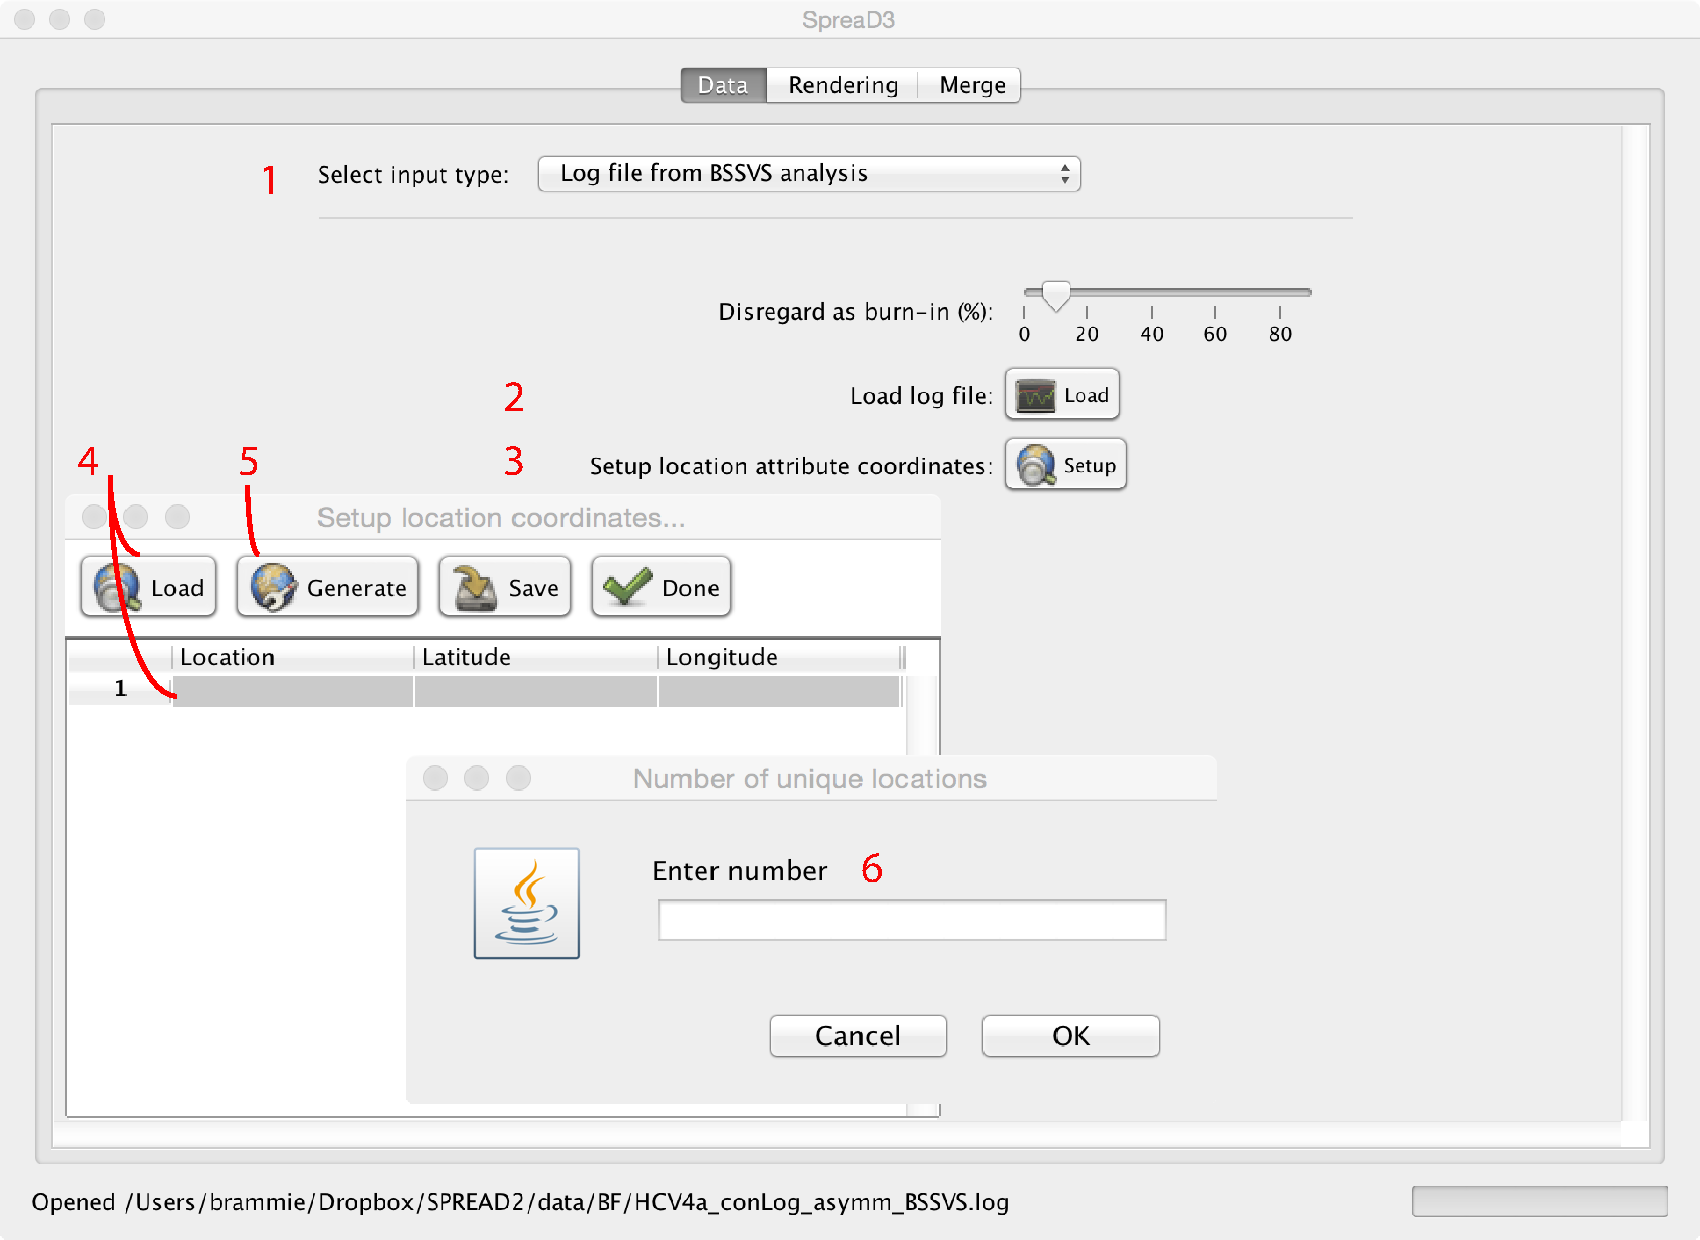
\includegraphics[width=1\textwidth]{./figures/Fig5_BFparse.pdf} %[scale=0.22]
\caption{Parsing options for the BSSVS analysis}
\label{fig:parseBF}
\end{figure}

\begin{figure}[!H]
\centering
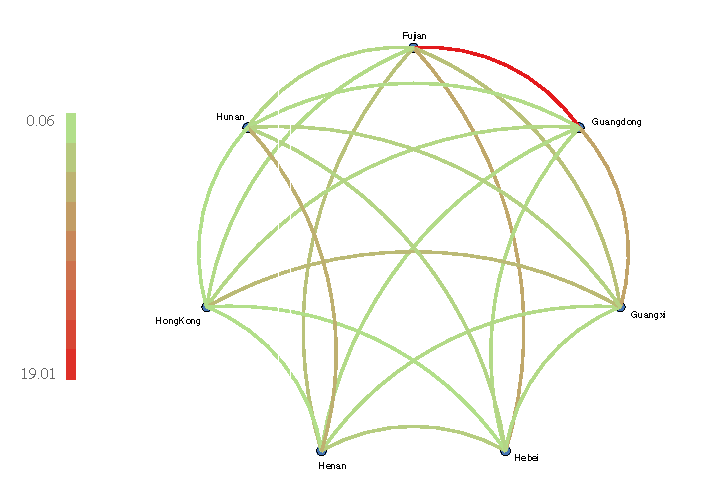
\includegraphics[width=1\textwidth]{./figures/bf_circle_final.pdf} %[scale=0.22]
\caption{Circle representation of the Bayes factor support for the possible location transitions for the H5N1 dataset}
\label{fig:BFcircle}
\end{figure}

\begin{figure}[!H]
\centering
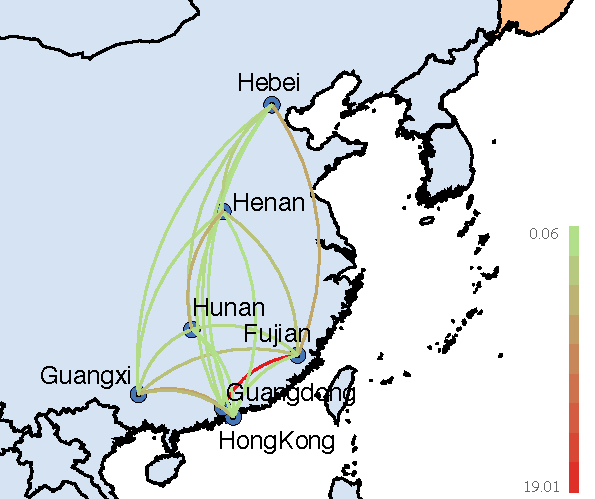
\includegraphics[width=1\textwidth]{./figures/bf_map_final.pdf} %[scale=0.22]
\caption{Bayes factor support for the possible location transitions for the H5N1 dataset overlaid on a geographical map}
\label{fig:BFmap}
\end{figure}



\subsection{Visualising a MCC tree annotated with continuous traits}
\label{MCCcontinuous}

For the example using an MCC tree annotated with continuous traits we revisit the work of \citet{Bouckaert:2012aa} in which the origin and spread of Indo-European languages was investigated with well-established phylogenetic methods.
We will here use the MCC tree summary to visualise their origin in and spread from Anatolia (a region in present day Turkey). 
This maps all branches of a continuous diffusion phylogeographic reconstruction and allows plotting the uncertainty of geographic coordinates at the internal nodes through their annotated highest posterior density contours.

\subsubsection{Parsing the data}
\label{MCCcontParse}

In the Data tab, select `MCC tree with CONTINUOUS traits' and browse to where the example tree is saved (Figure \ref{fig:parseMCCcont}, nr 1).
Because the latitude and longitude are by default annotated as `trait1' and `trait2' by BEAST, we adhere to this ordering and first provide the y-coordinate (latitude, trait1), and than the x-coordinate (longitude, trait2) (Figure \ref{fig:parseMCCcont}, nr 2).
The option `External annotations' %perhaps change to `External branch annotations' 
is to be used when the child node trait values have an associated uncertainty (Figure \ref{fig:parseMCCcont}, nr 3).
Because the locations at the tips in this example cover the areas where the language is spoken this options should be selected.
On the other hand, one can safely ignore this option whenever the tips traits have no associated uncertainty (e.g. exact longitude and latitude). 
When the MCC tree is annotated with multiple levels of trait uncertainty (that is, multiple HPD levels), the level of interest can be chosen (Figure \ref{fig:parseMCCcont}, nr 4).
The provided example tree only has 1 HPD level annotation (80\%).
You can leave the most recent sampling date for this example to its default value, just as the Time scale multiplier (Figure \ref{fig:parseMCCcont}, nr 5).
To conclude the parsing step, select the world.geojson file and generate `language.json' (Figure \ref{fig:parseMCCcont}, nr 6 and 7.

\begin{figure}[!H]
\centering
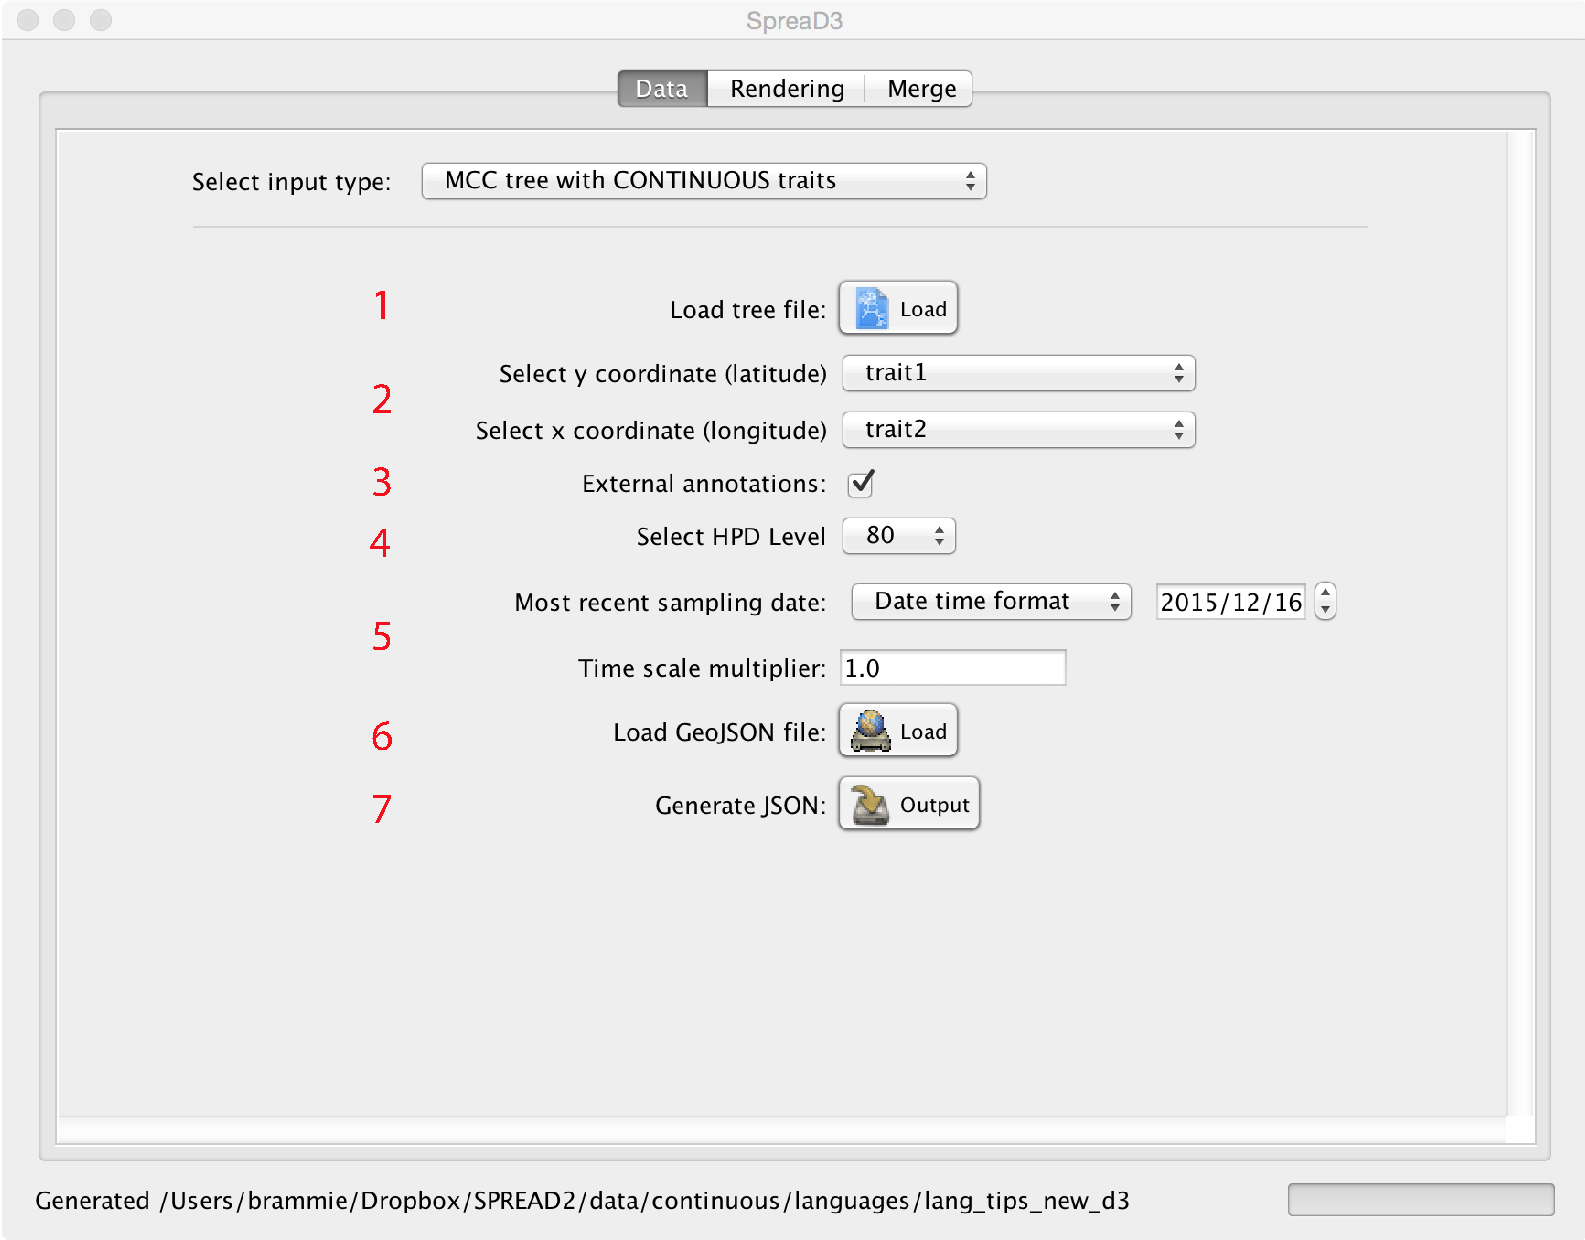
\includegraphics[width=1\textwidth]{./figures/new_parse_cont_language.pdf} %[scale=0.22]
\label{fig:parseMCCcont}
\caption{Parsing options for the `MCC tree with continuous traits' analysis}
\end{figure}

\subsubsection{Rendering and specifying the visualisation options}

Open the Rendering tab, load language.json and save as language\_D3 (Figure \ref{fig:renderMCCcont}).
As before, we start by giving the geographical map on which the tree is projected an appropriate color. 
Let's keep the white color for the seas, and contrast this with grey for the land masses. % de gustibus et coloribus ...
For this, set the Map fill color to \#000000 and the Map fill opacity to 0.2. 
Note that, depending on the loaded geoJSON map, this may also be achieve by selecting the appropriate Map fill attribute. 
Next, color the Points and Lines according to the time.
For this, set the Point/Line color attribute to height (measured from the tips to the root), and the start and end color to respectively \#a6cee3 and \#cab2d6.
Finally, let's visualise the uncertainty on the internal nodes by setting the Polygon color attribute to `posterior'.
By setting the start color to light orange (color code \#fdbf6f) and the end color to green (color code \#b2df8a), nodes with higher posterior support will be surrounded by progressively more intense green polygons.
Try several values for  the Polygon opacity to see how this affects the 
To include the legend in the image, print the web page and copy-paste the legend in the image with e.g. Illustrator. 

\begin{figure}[!H]
\centering
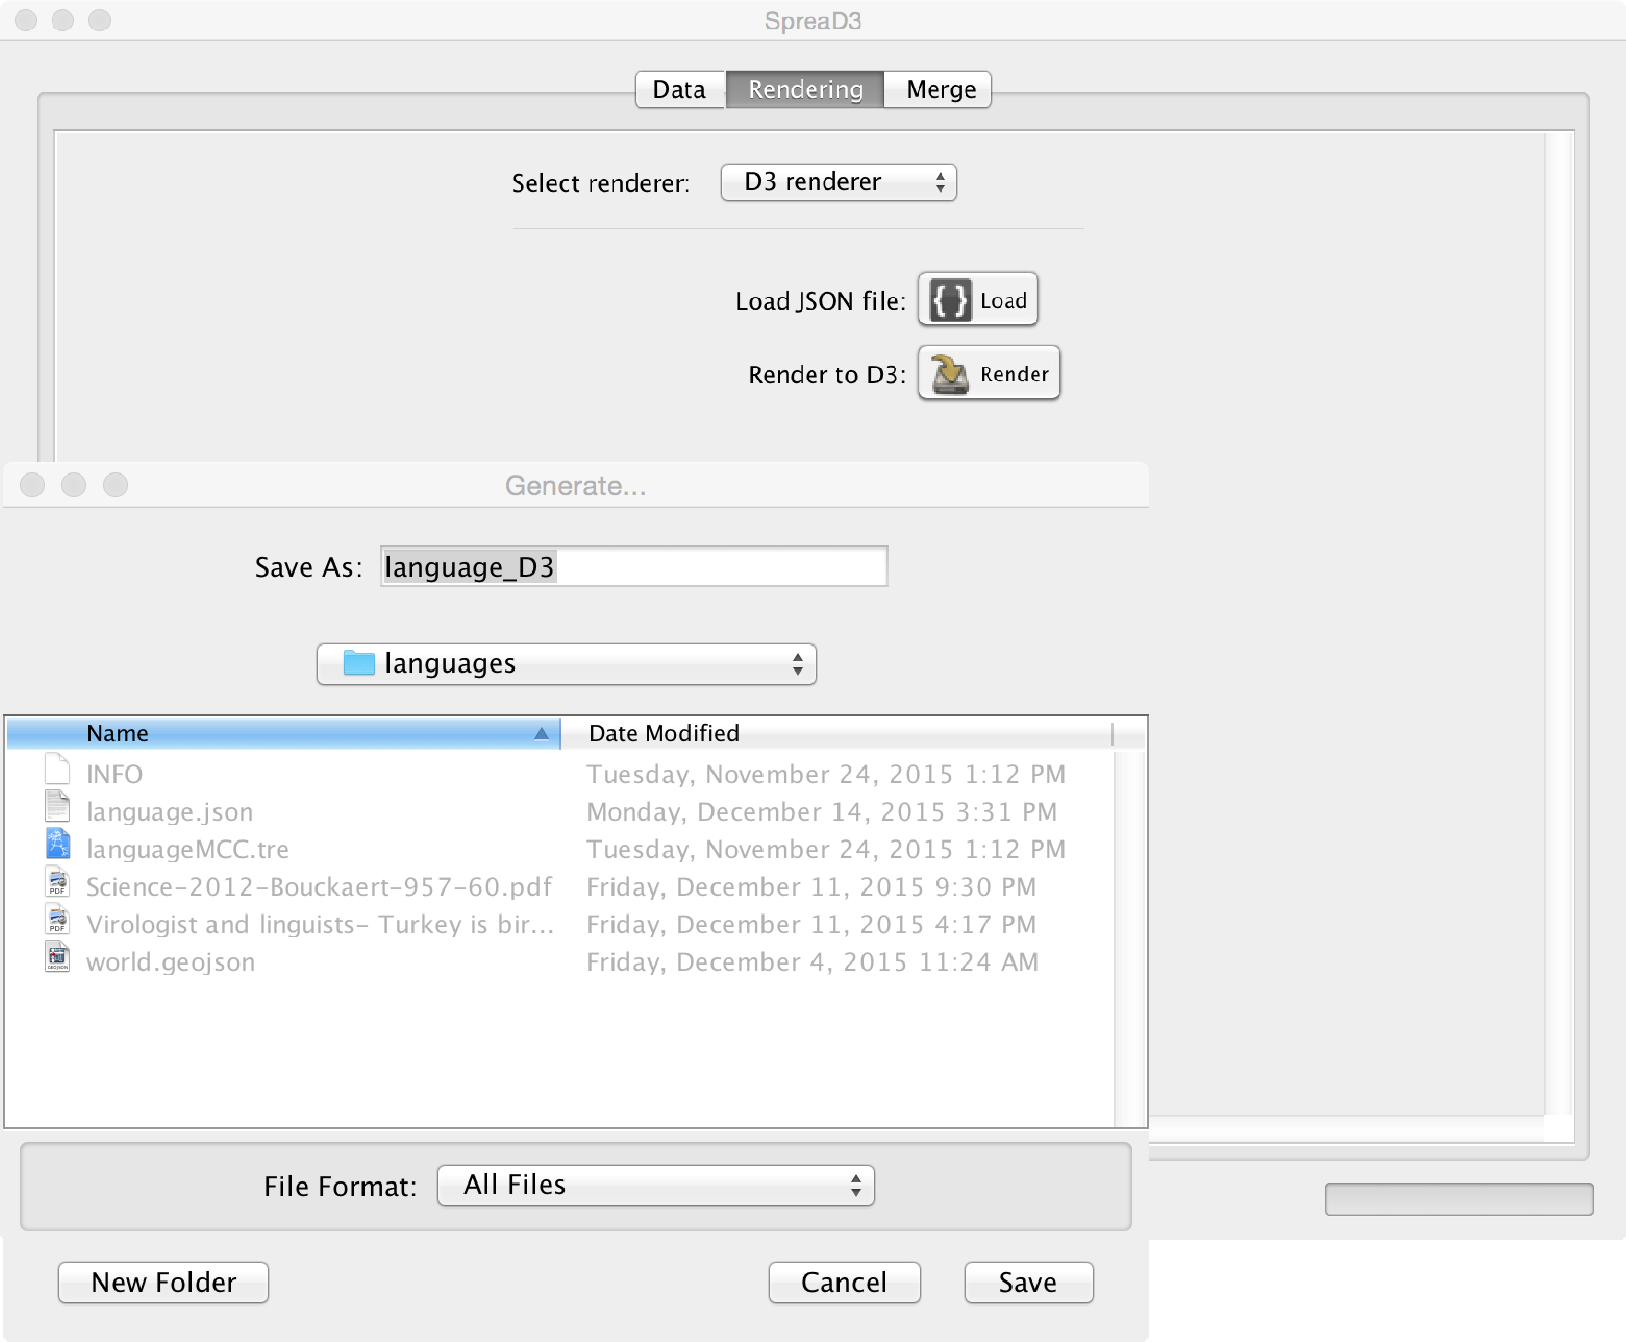
\includegraphics[width=1\textwidth]{./figures/Fig4_continu_render} 
\caption{Rendering options for the `MCC tree with continuous traits' analysis}
\label{fig:renderMCCcont}
\end{figure}

\begin{figure}[!H]
\centering
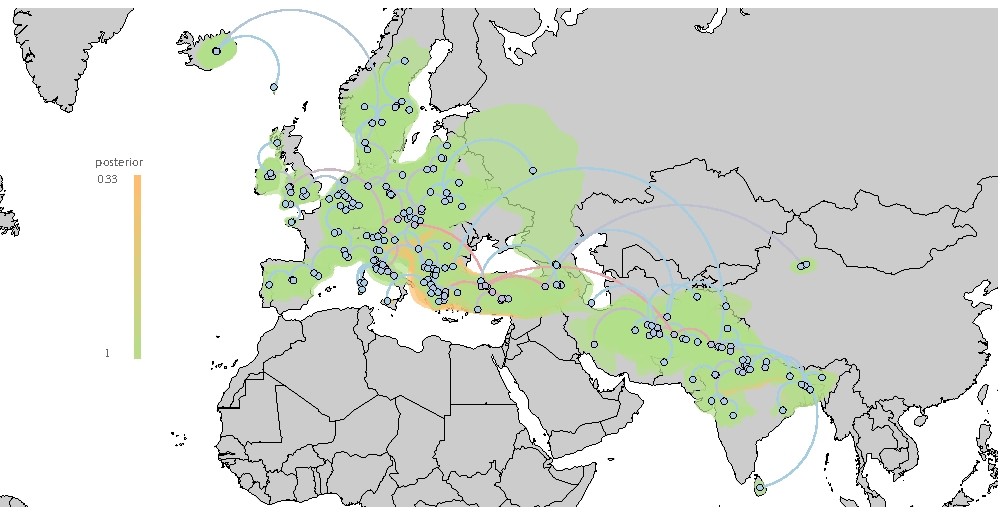
\includegraphics[width=1\textwidth]{./figures/new_image_cont_language.pdf} 
\label{fig:imageMCCcont}
\caption{{\spreadname} generated image of the language dataset from \citet{Bouckaert:2012aa}}
\end{figure}


\subsection{Visualising a distribution of trees annotated with continuous traits}
\label{contTreeDistr}
% 2.4 time-slicing 
% - West Nile Virus as an example?
% - show how one can use MCC tree to generate the slices or define
% his/her own slice heights
% - merge continuous tree with JSON file resulting form time slicing a
% posterior distribution for a joint visualisation.
% 

For this example we use the West Nile virus dataset previously analysed by \citet{Pybus:2012aa}.
%much copy-paste from old tuto:
This analysis allows one to summarise and visualise the full posterior distribution of trees obtained in continuous phylogeographic analysis. 
To achieve this {\spreadname} creates a time line by slicing through each phylogeny at particular points in time, and imputes the unobserved descendant locations for those ancestral infections.
Uncertainty on these estimates is reflected by contouring them with polygons, which provides a natural representation of the uncertainty in these inferences. 
%how are the time slices chosen/determined?

\subsubsection{Parsing the data}

Select `Tree distribution with CONTINUOUS traits' from the Data tab, load the trees, set the 2D trait to `location' and load the MCC tree summary 
(Figure \ref{fig:parsePosterior}, nr 1, 2 and 3).
The time slices are based on the MCC tree length, but it is also possible to supply a file with custom slice heights in a single column and in ascending order (from the tips to the root of the phylogeny) . 
For this, set `time slices' to Custom (Figure \ref{fig:customTimeSlices}, nr 1) and load the time slice file (Figure \ref{fig:customTimeSlices}, nr 2).
The most recent sampling tine in this dataset is 2007.63 - reset the data format to decimal 
(Figure \ref{fig:parsePosterior}, nr 4).
The trees distribution has been subsampled with LogCombiner (a tool distributed with BEAST) to reduce its size, at which stage the burnin was removed. 
Hence, set the burnin to zero 
(Figure \ref{fig:parsePosterior}, nr 5).
Leave the other options at their default values, select the provided geojson map (Figure \ref{fig:parsePosterior}, nr 6) and generate wnv\_trees.json.
Because the trees-file is rather large this may take a few moments.
\par
We also visualise the MCC tree which gave rise to the time slices by drawing its branches.
For this, parse the West Nile virus MCC tree as before and save as wnv\_mcc.json (Figure \ref{fig:parsePosteriorMCC}).
Before rendering, the time slice JSON file and the MCC tree JSON file need to be combined.
Open the `Merge' tab and double click in the `Choose file\dots' box to browse to and load the JSON files (Figure \ref{fig:mergeTimeSlice}, nr 1).
To add a JSON file, select the `+' button in the bottom left corner of the screen (Figure \ref{fig:mergeTimeSlice}, nr 2).
Keep the Points and Lines layers from wnv\_cc.json, and the other layers from wnv\_trees.json (Figure \ref{fig:mergeTimeSlice}, nr 3).
To save the merged file as ag\_combined.json, select File $\rightarrow$  Merge. 

\begin{figure}[!H]
\centering
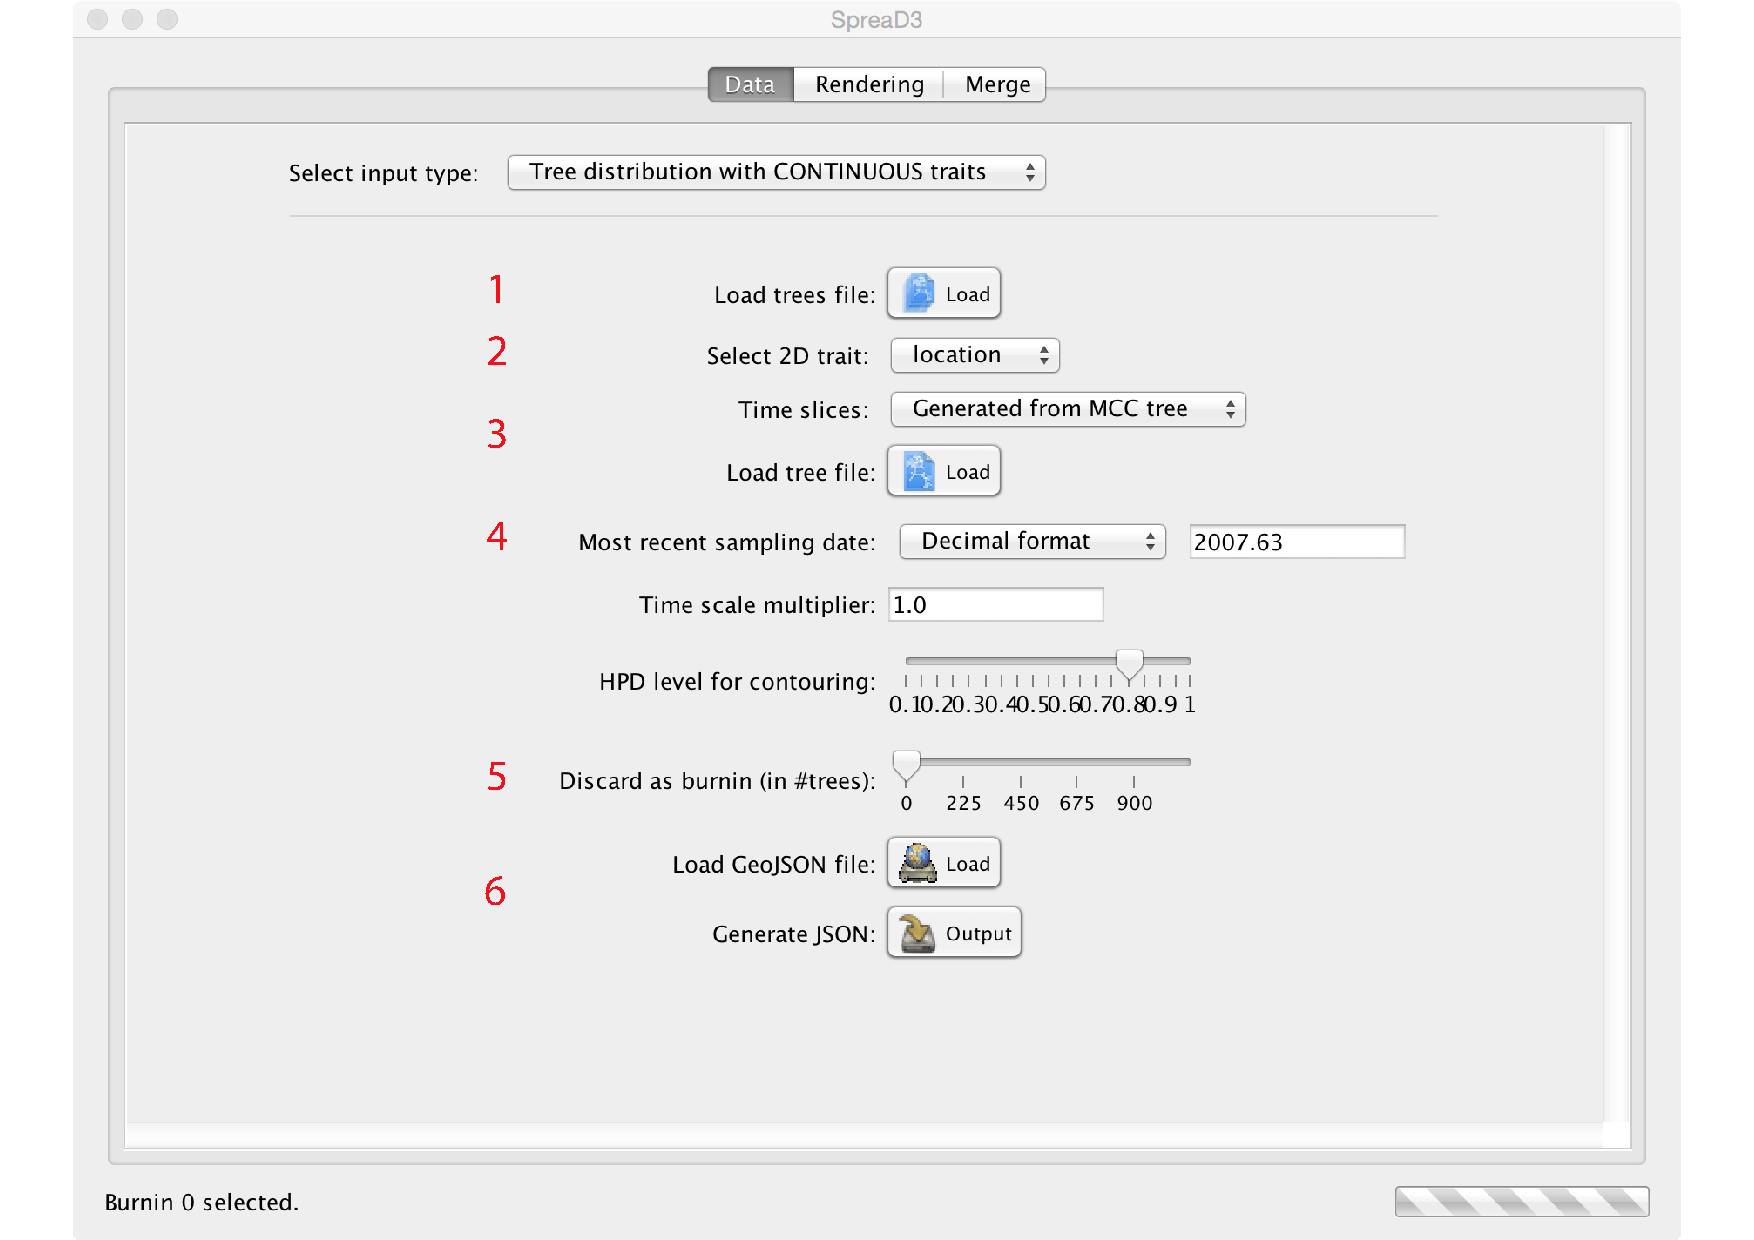
\includegraphics[width=1\textwidth]{./figures/Fig_parseTrees.pdf} 
\caption{Parsing options for the `Tree distribution with continuous traits' analysis}
\label{fig:parsePosterior}
\end{figure}

\begin{figure}[!H]
\centering
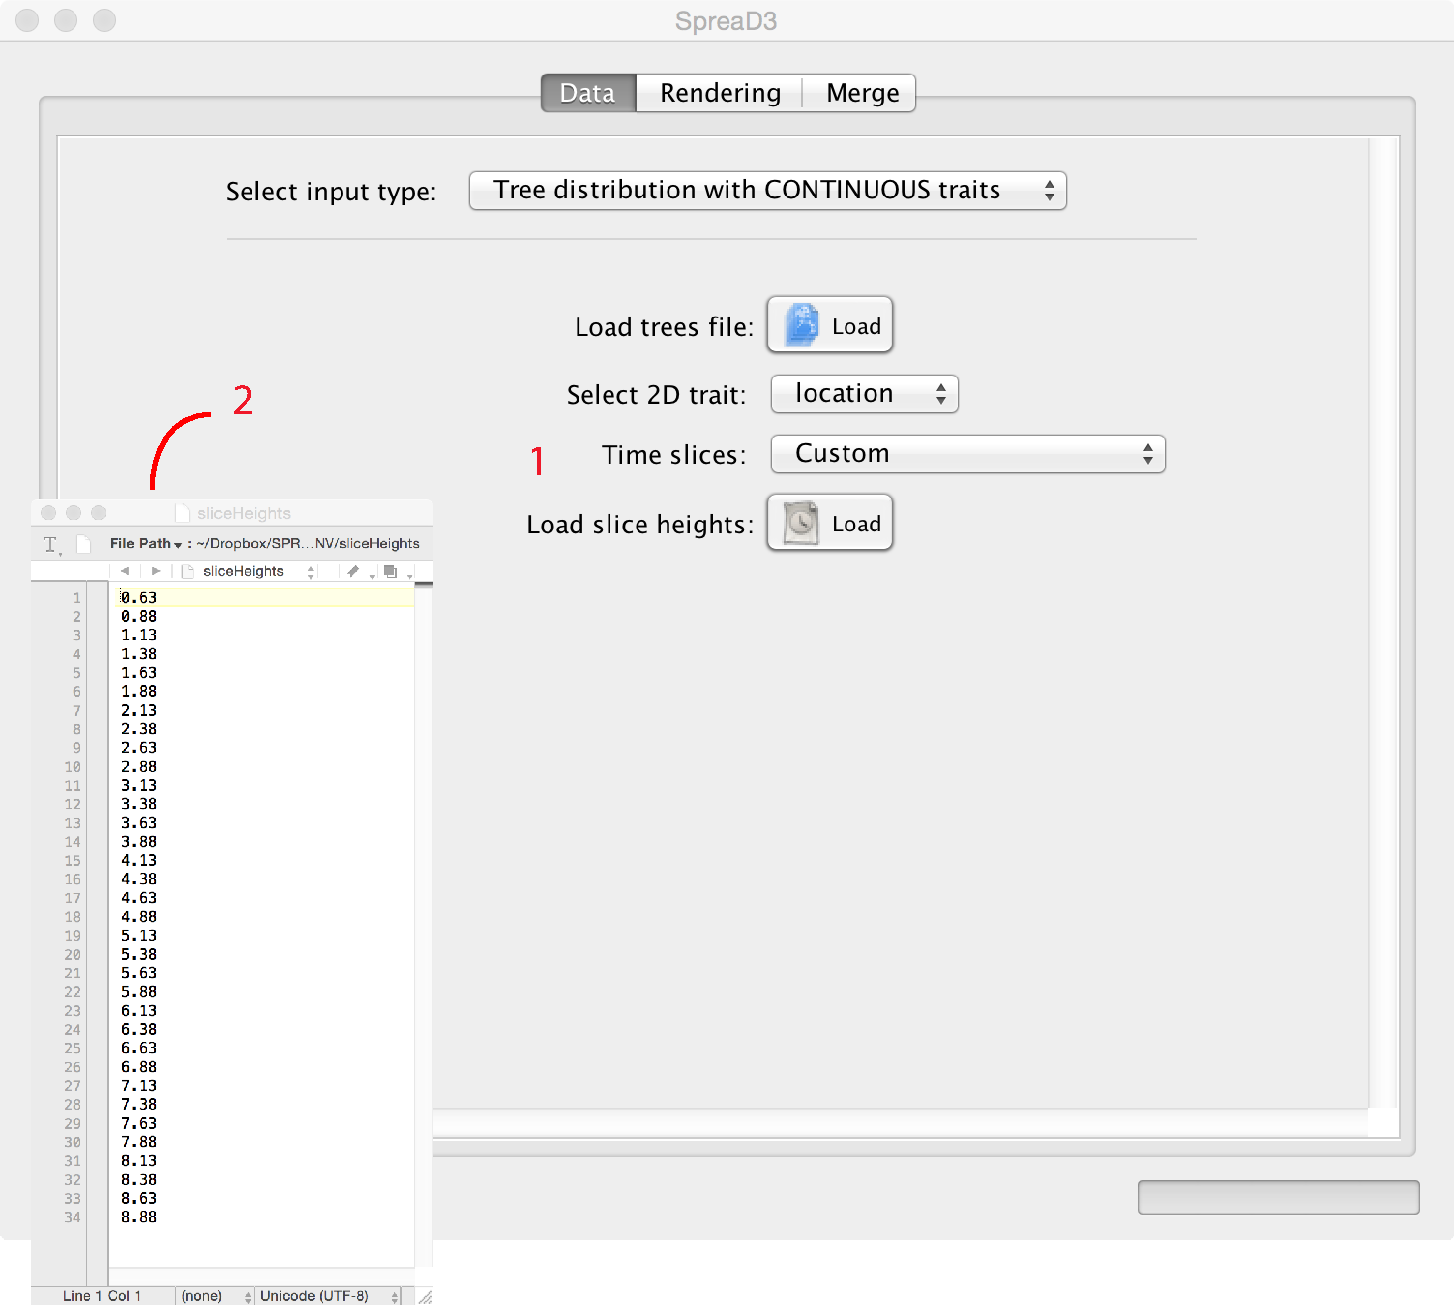
\includegraphics[width=1\textwidth]{./figures/customTimeSlices.pdf} 
\caption{Specifying custom time slices}
\label{fig:customTimeSlices}
\end{figure}


\begin{figure}[!H]
\centering
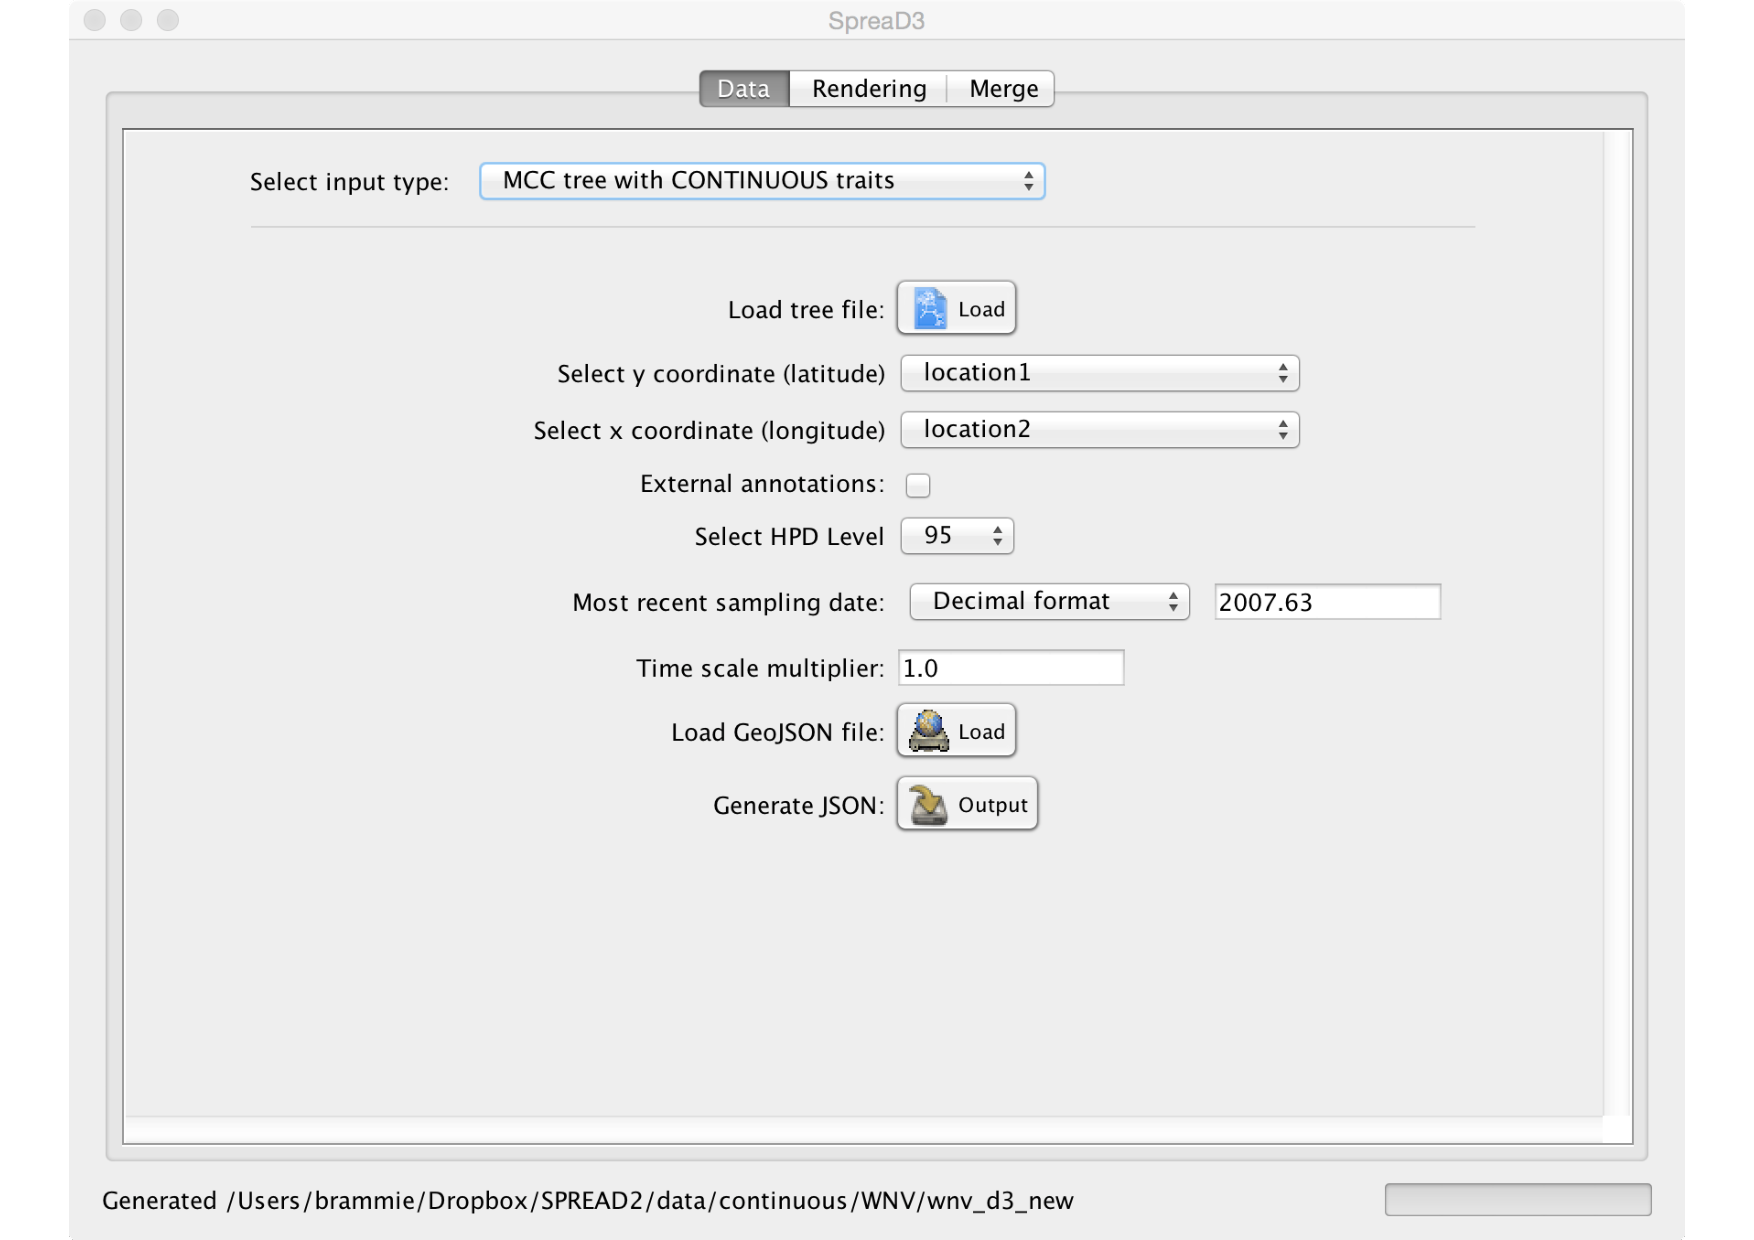
\includegraphics[width=1\textwidth]{./figures/new_parseMCCposterior.pdf} 
\caption{Parsing options for the `MCC tree with continuous traits' analysis}
\label{fig:parsePosteriorMCC}
\end{figure}

\begin{figure}[!H]
\centering
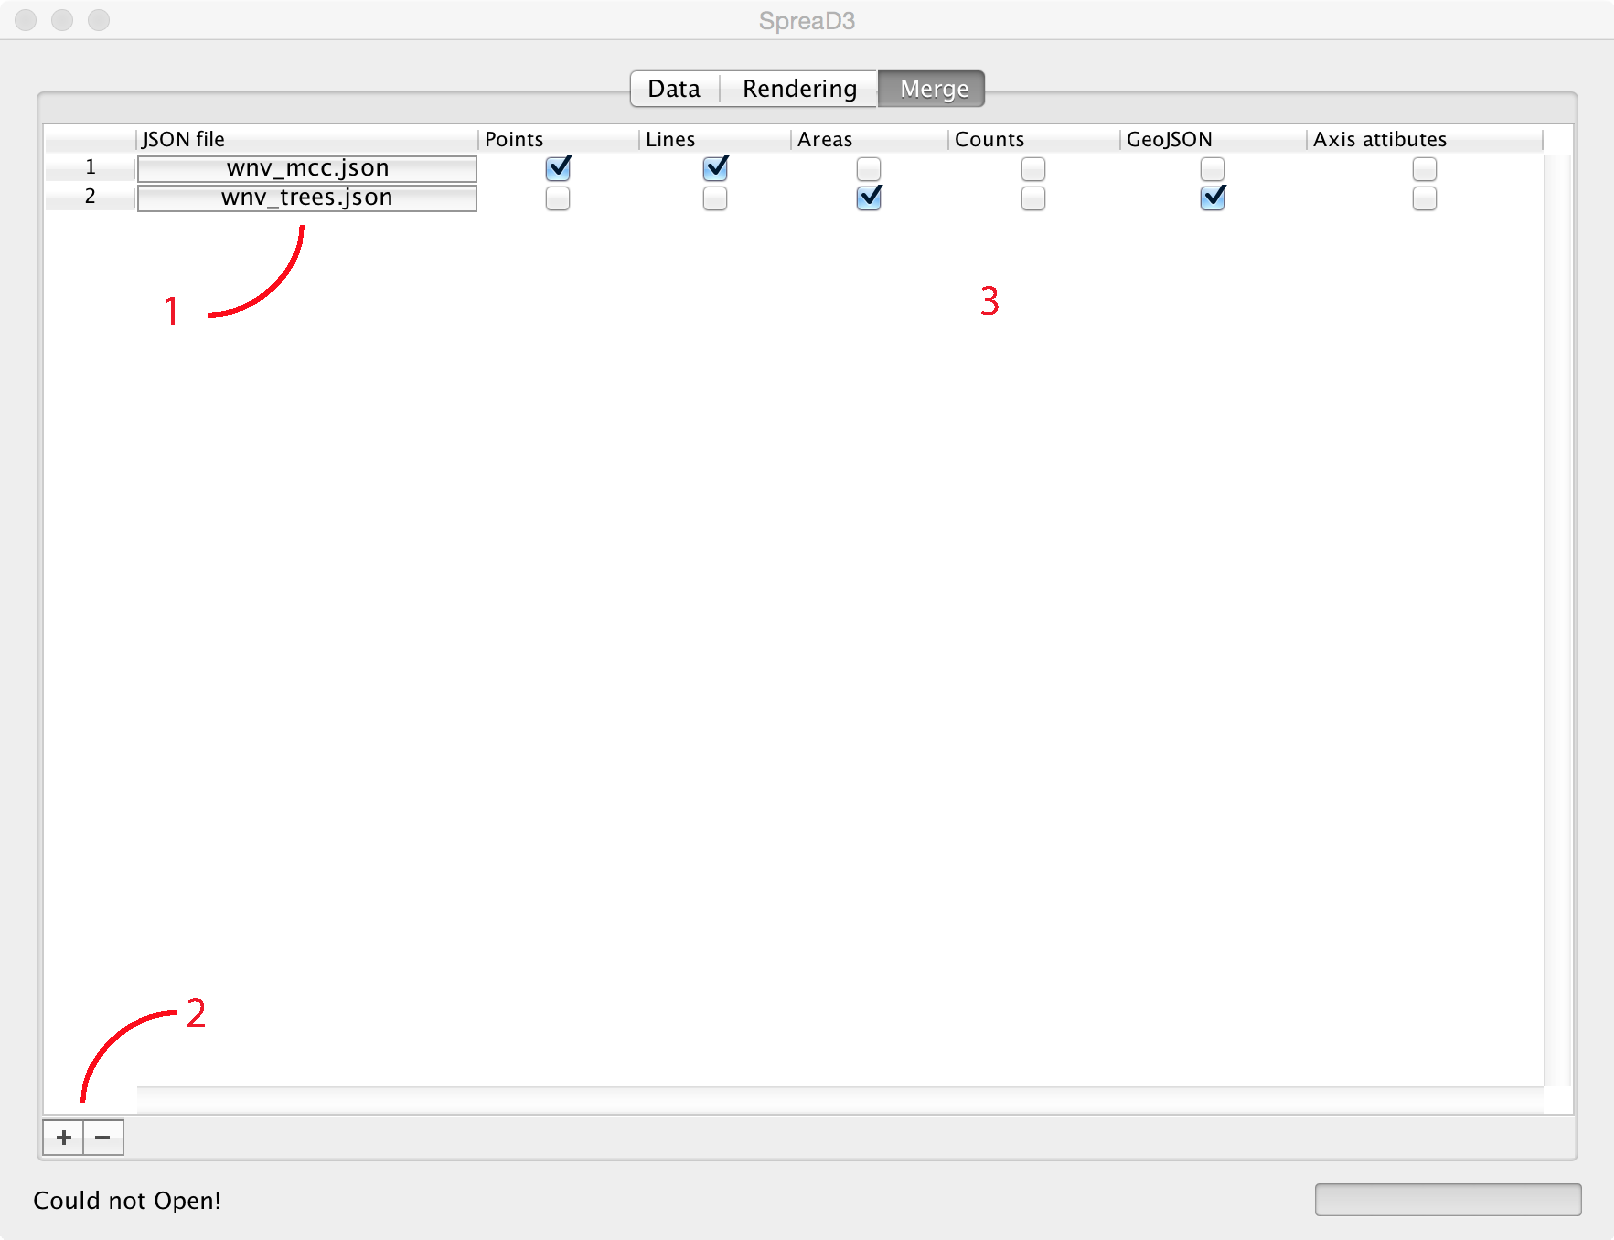
\includegraphics[width=1\textwidth]{./figures/new_merge_wnv.pdf} 
\caption{Example of merging the desired layers of various {\spreadname} parsing outputs}
\label{fig:mergeTimeSlice}
\end{figure}


\subsubsection{Rendering and specifying the visualisation options}

There are only a few steps required to arrive at the final image for this example (Figure \ref{fig:TimeSliceFigure}).
First give the seas a grey colour by setting the Backgound color to grey.
Next, colour the land mass dark grey by setting the Map color to black (colour code \#000000) and the Map fill opacity to .7.
Update the colour of the contours: set the Polygon color  to \#74add1 and the Polygon opacity to .4.
Finally, color the poins and lines by the time by setting the Poins/Lines color attribute to `heigth', and their start and end colours to \#b2df8a and \#fdbf6f respectively.

\begin{figure}[!H]
\centering
% FB: uncommited figure? BV: idd
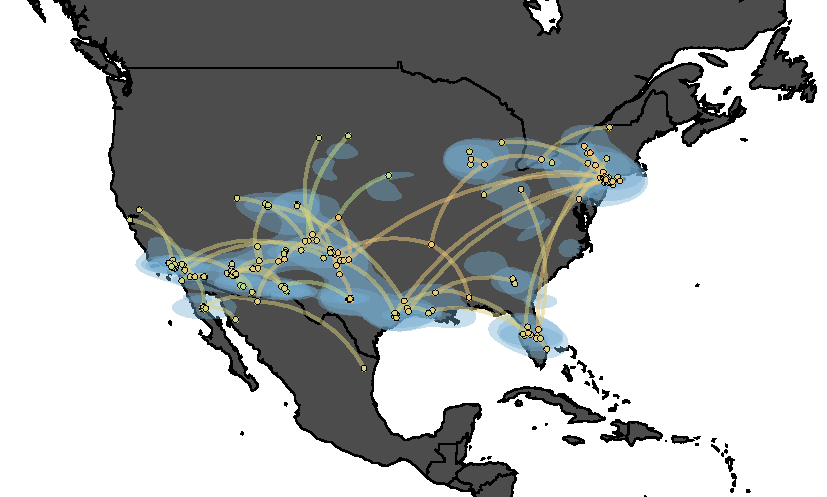
\includegraphics[width=1\textwidth]{./figures/Fig_WNVout.pdf} 
\caption{{\spreadname} generated image of the West Nile virus dataset from \citet{Pybus:2012aa}}
\label{fig:TimeSliceFigure}
\end{figure}


\subsection{Tips \& tricks\label{sub:tips}}

% Tips & Tricks
%  - we should show the antigenic coordinates example here, where the
% coordinates are other than lat/long and there's no underlying map. I
% also have the multiple HPD's example, on which we can sho whow the
% merging works. W parse 3 JSONs for all HPD levels, merg ethem and
% jointly visualise, coloring polygons by HPD levels.
% - antigenic coord (or any other trait for taht matter) coul dbe plotted as a function of time (height attribute)
% - nodes/ branches of a given tree can be anotated in Figtree, these
%   values can then be used as a basis for mapping
% 
% - Some examples of KML rendering, using previously generated JSON files,
%   just to show that we still support it.

We illustrate the use of {\spreadname} for data mapped to other coordinates than longitude and latitude with an antigenic coordinate ancestral reconstruction for an influenza A/H3N2 virus dataset taken from \citet{Bedford:2014aa}.
Antigenic distances are a quantitative measure of how antigenically dissimilar virus strains are, and are projected on a 2D map.
When no underlying map is provided, {\spreadname} simply draws a bounding box around the data points.
The idea here is to visualise three layers of uncertainty by combining the polygons of the 50\%, 75\% and 95\% Highest Posterior Density interval.

\subsubsection{Parsing the data}

The parsing is fully analogous to the parsing explained in \ref{MCCcontParse}, with the exception that the x and y coordinates now are antigenic1 and antigenic2 respectively.
Don't forget to select `External annotations' (Figure \ref{fig:parseTipsTricks}, nr 1 and 2). 
Save the files as `ag\_95.json', `ag\_75.json' and `ag\_50.json' (one output file per HPD annotation). 
Now combine these files (Figure \ref{fig:mergeTipsTricks}) and save as `ag\_combined.json.

\begin{figure}[!H]
\centering
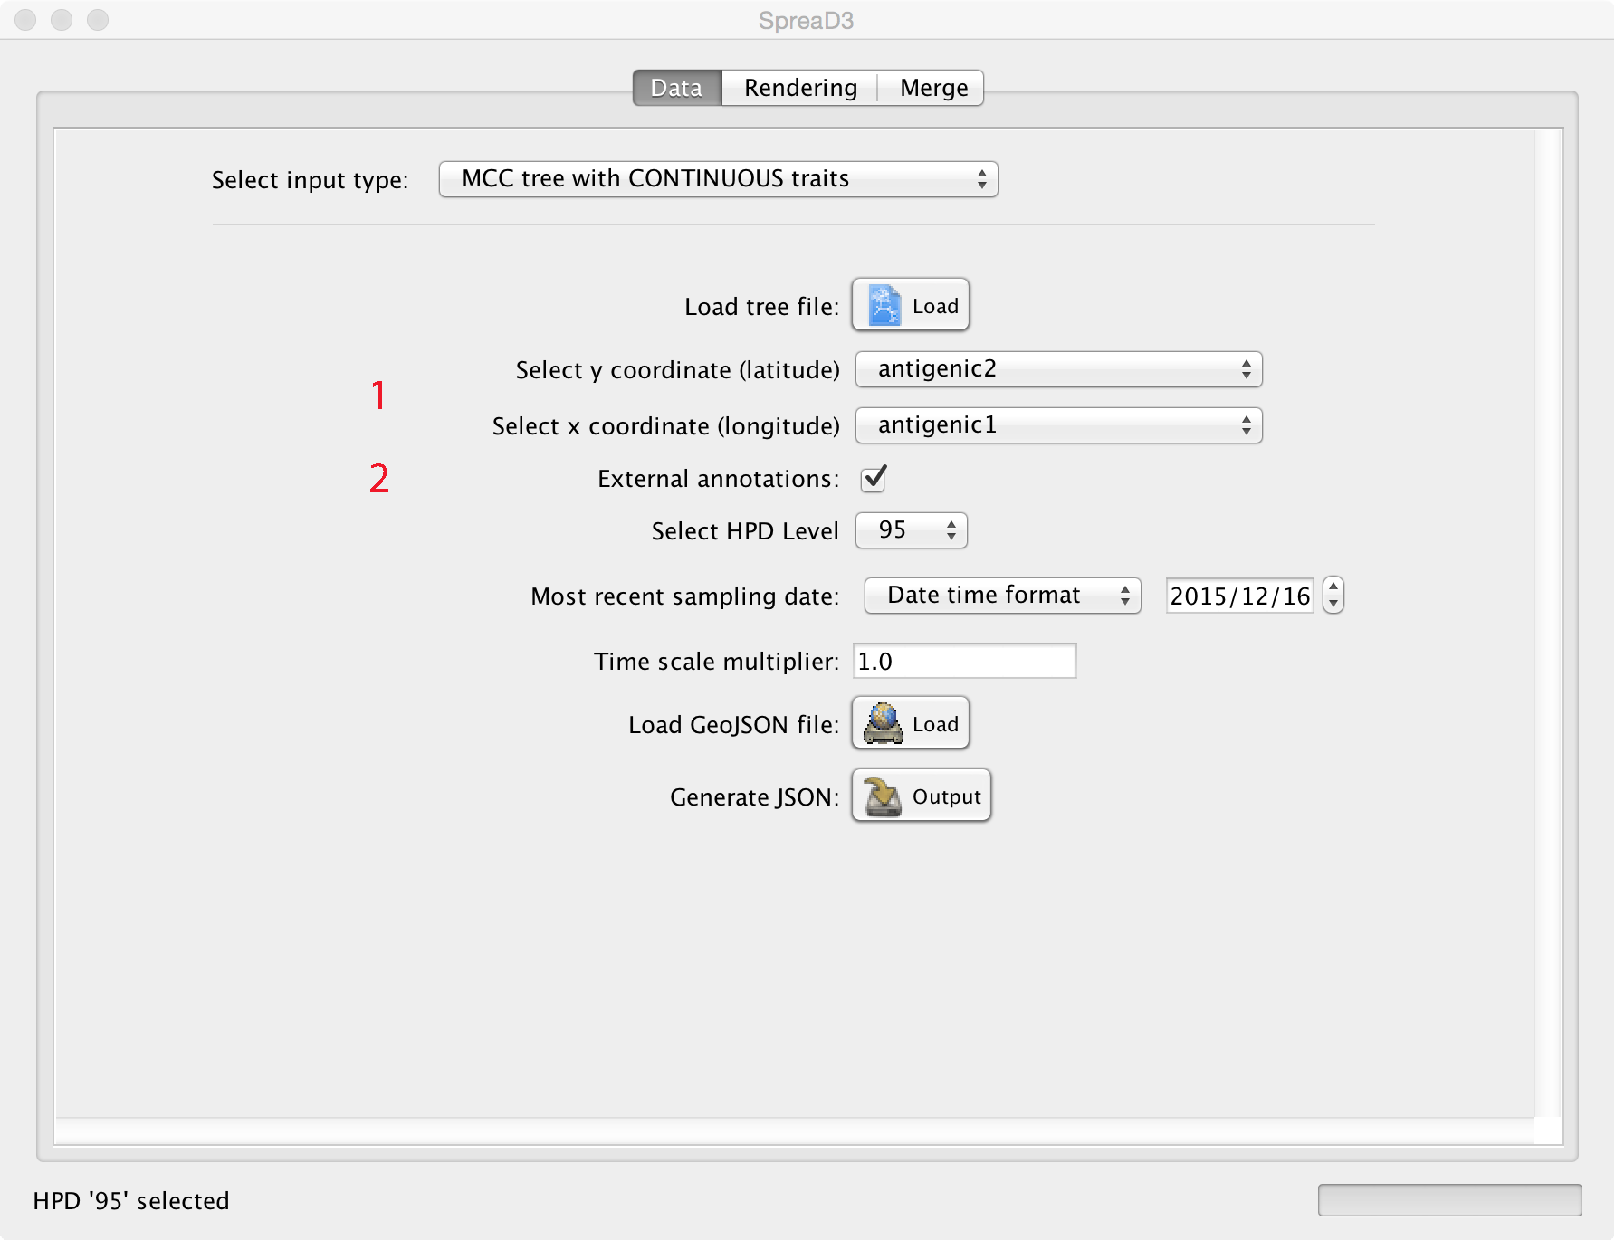
\includegraphics[width=1\textwidth]{./figures/new_ag_parse.pdf} 
\caption{Parsing options for the `Tree distribution with continuous traits' analysis}
\label{fig:parseTipsTricks}
\end{figure}

\begin{figure}[!H]
\centering
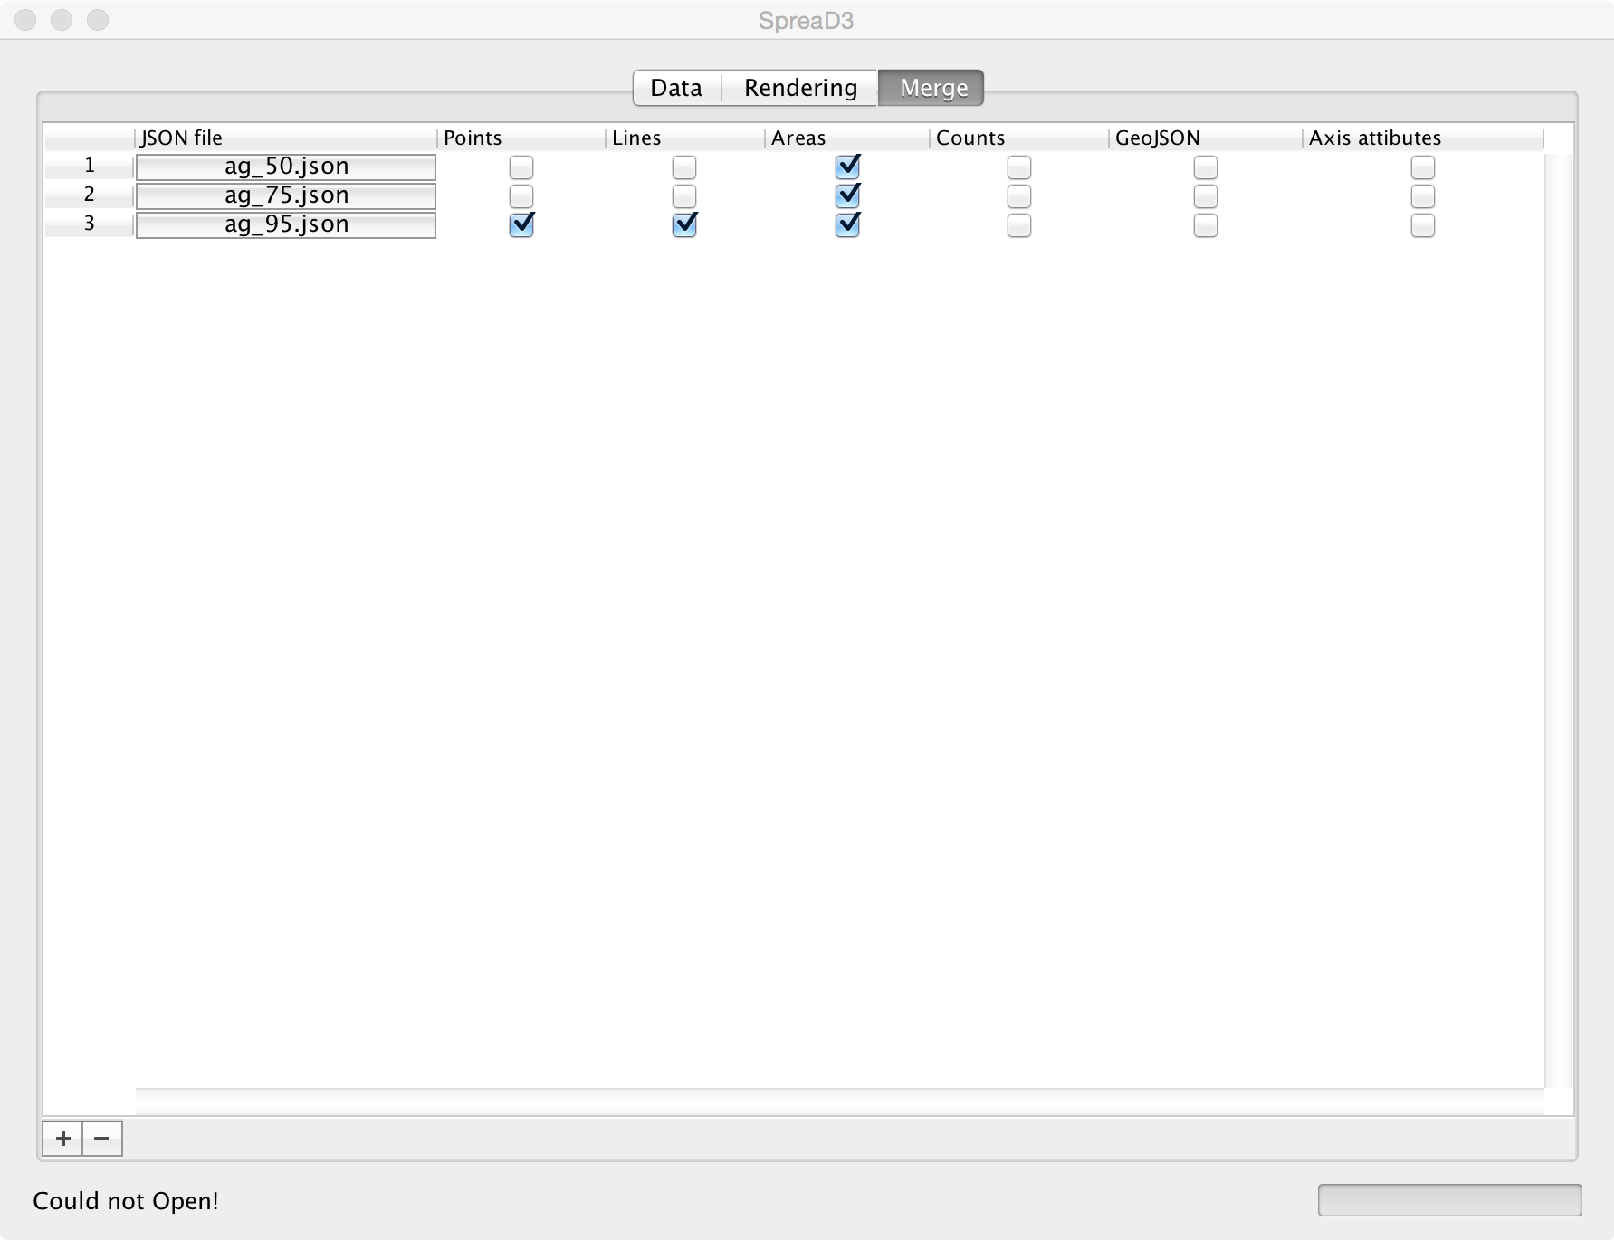
\includegraphics[width=1\textwidth]{./figures/new_merge_ag.pdf} 
\caption{Example of a merging the desired layers of various {\spreadname} parsing outputs}
\label{fig:mergeTipsTricks2}
\end{figure}

\subsubsection{Rendering and specifying the visualisation options}

Do the following to obtain Figure \ref{fig:mergeTipsTricks}.
Set the Line color attribute to antigenic1 and its start and end colors to \#1f78b4 and \#fb9a99 respectively. 
Do the same for the Point color attribute.
The HPD layers, which take 3 discrete values, can be given a separate colour by setting the Polygon attribute color to HPD.
Lower the Polygon opacity to .1 to visualise the contours of the wider HPDs.

\begin{figure}[!H]
\centering
\includegraphics[width=1\textwidth]{./figures/map_ag.pdf} 
\caption{The antigenic coordinate map with three layers of uncertainty (50\%, 75\% and 90\% HPD intervals)}
\label{fig:mergeTipsTricks}
\end{figure}

Changing the start and end colors of the Polygon attribute color via the GUI has no effect because the HPD attribute is a categorical variable rather than a continous one. 
However, the color palettes\footnote{Example of color palettes can be found at \url{http://bl.ocks.org/mbostock/5577023}} can be changed using the Java Script command line.
In FireFox, this is accessible via the Webconsole (Figure \ref{fig:overridePalette}).
For example, to select a palette of blues, set 
\\
ordinalColors = colorbrewer.Blues[3];
\\
The changes take effect after toggling the attribute between another variable and HPD.
Note that the color scheme for continuous variables and fixed values can also be manually set in this way.
E.g. for continuous variables the syntax is 
\\
pairedSimpleColors = colorbrewer.[Palette];
\\
and for fixed colors this becomes:
\\
fixedColors = colorbrewer.RdYlBu[11];
.

\begin{figure}[!H]
\centering
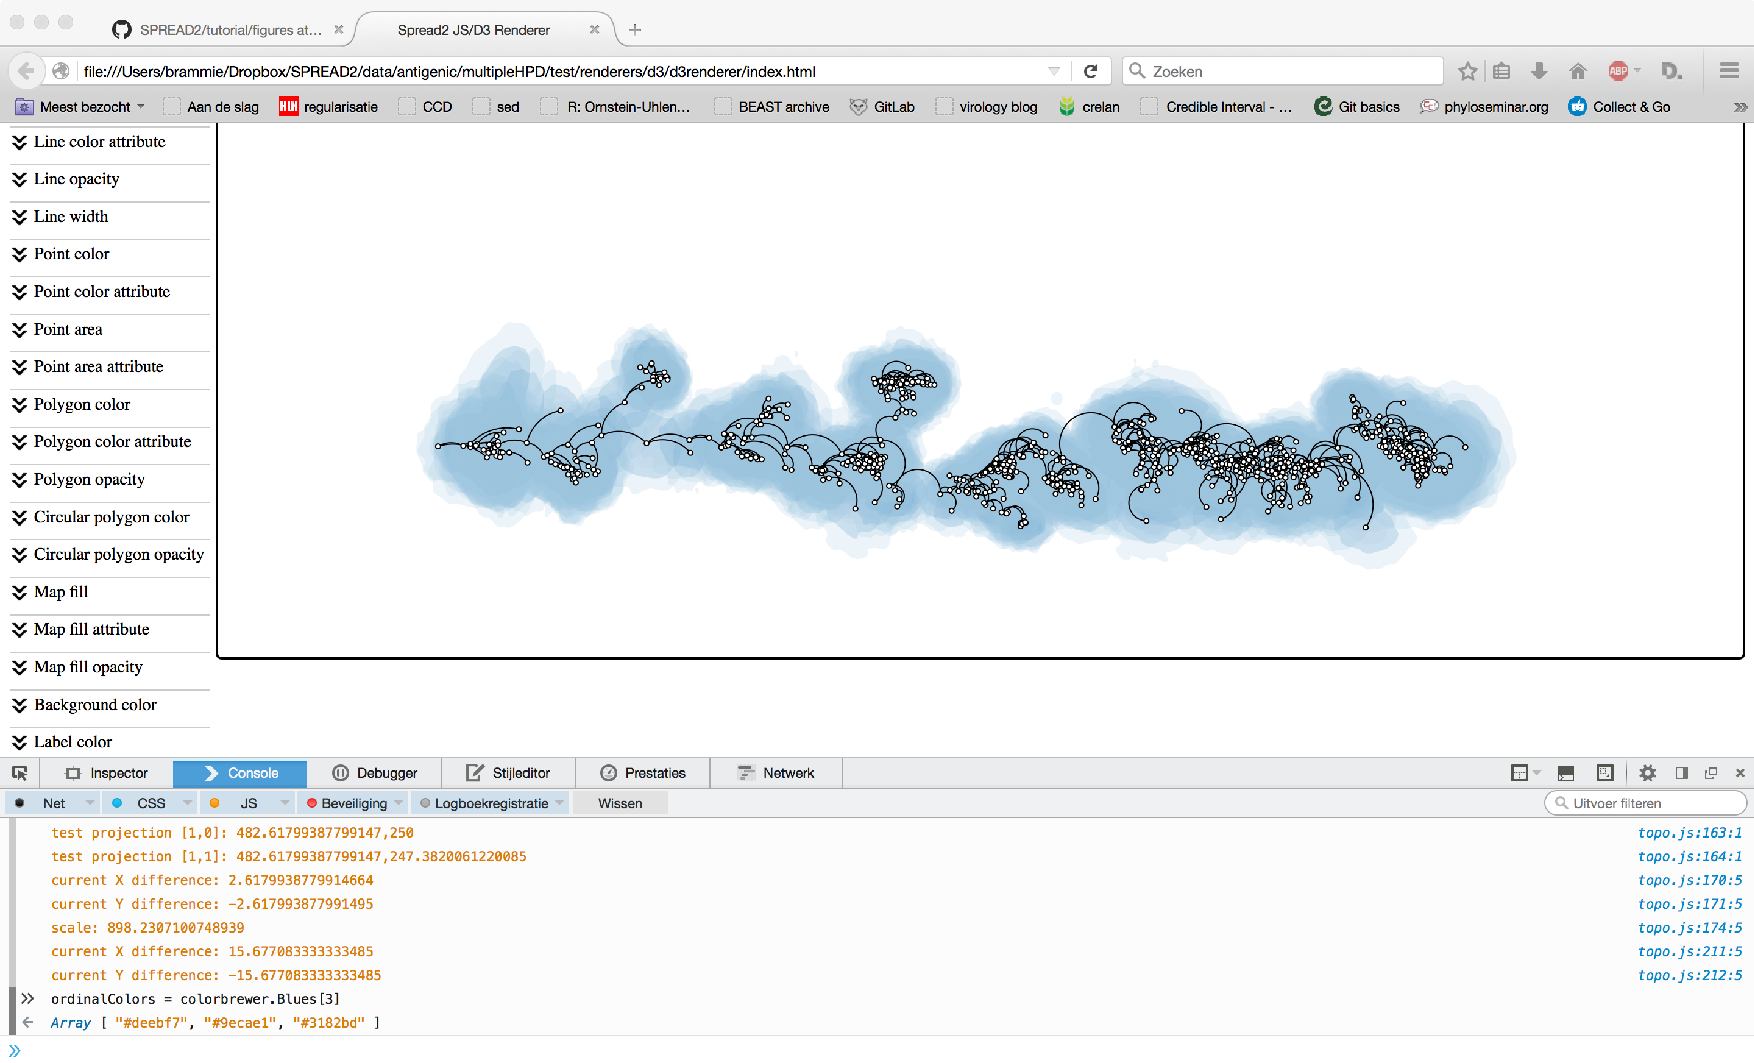
\includegraphics[width=1\textwidth]{./figures/manualOverride_palette.pdf} 
\caption{Illustration of how to manually set the color palette.}
\label{fig:overridePalette}
\end{figure}


\subsection{KML rendering}
\label{kmlRender}

The previously generated JSON files can also be used to render the images in KML. 
As an example, open ebov.json and select `render as KML'.
Several panels that enable the user to fine-tune the appearance of the elements used to represent all facets of the phylogeny and its associated traits appear\footnote{In some browsers the window needs to be resized a little to make these visualisation options appear.} (Figure \ref{fig:KMLrender}).
The output of this rendering can be viewed in virtual globe software (e.g. Google Earth).

\begin{figure}[h]
\centering
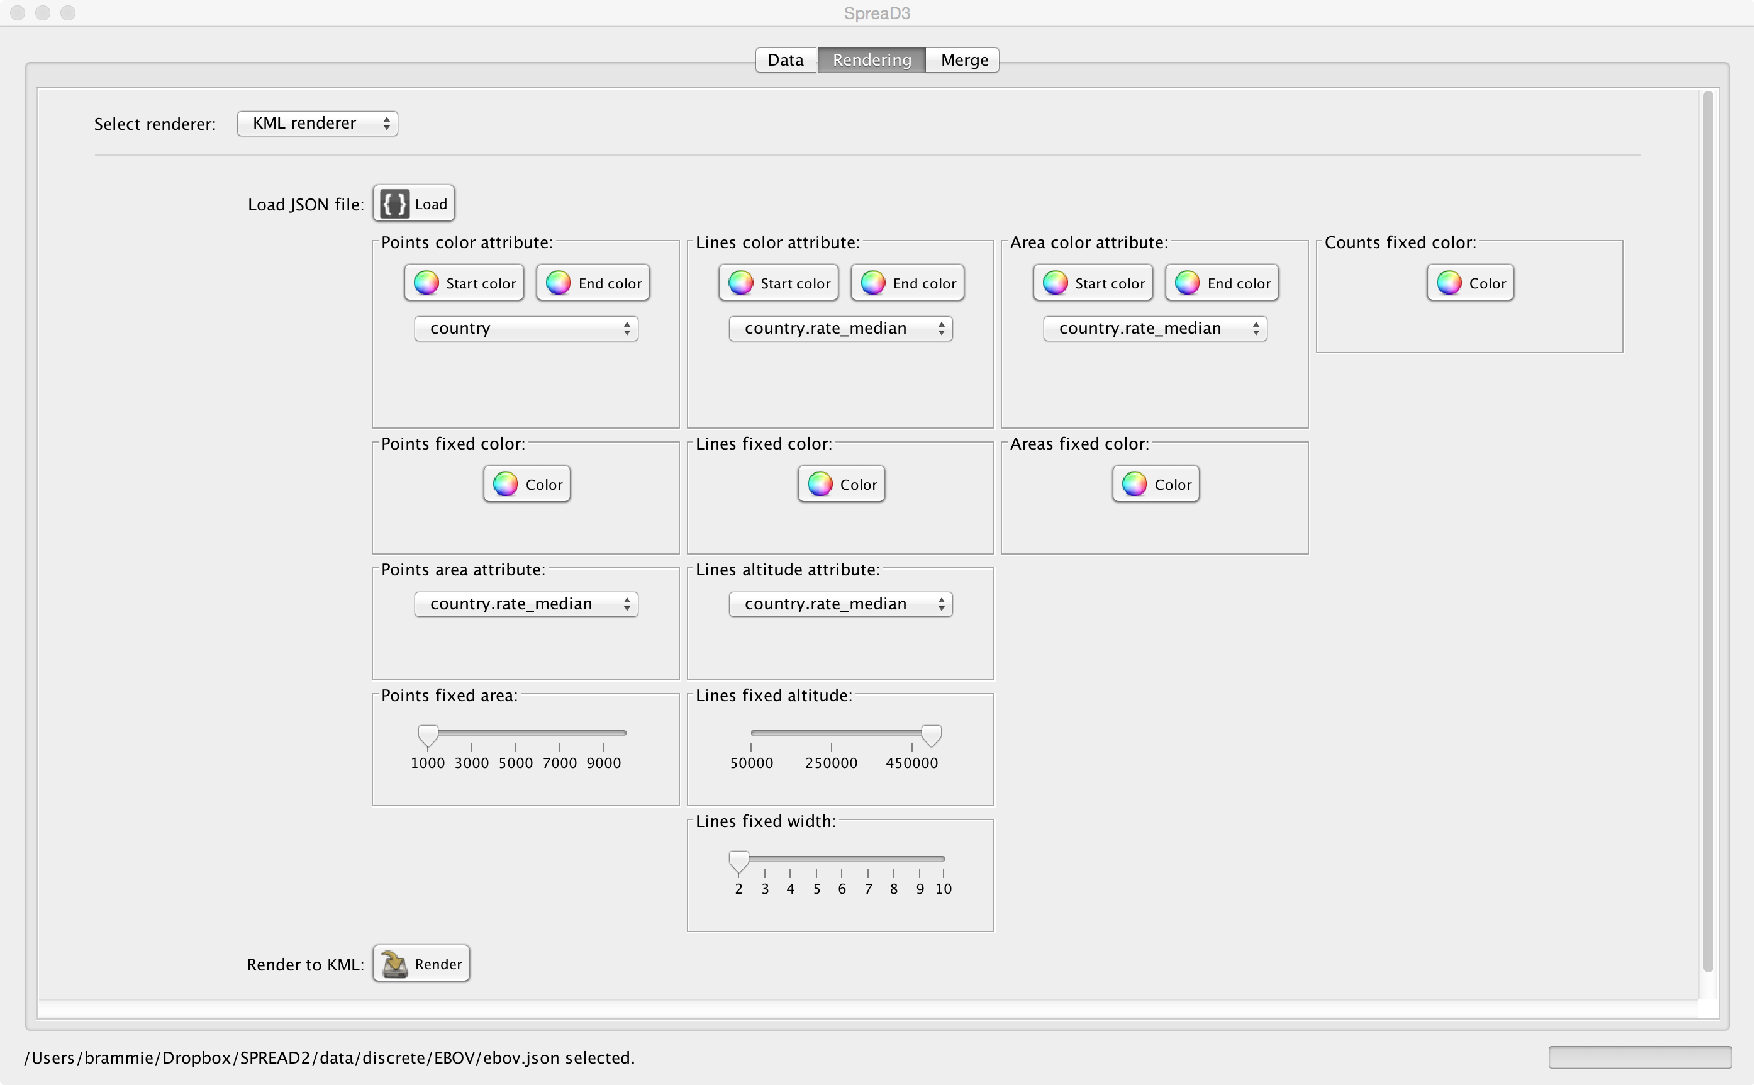
\includegraphics[width=1\textwidth]{./figures/kml_render.pdf} 
\caption{The visualisation options when rendering to KML}
\label{fig:KMLrender}
\end{figure}


\subsection{Command line interface\label{CLI}}

We have found it easiest to use the command line interface with an alias added to .bash\_profile:

\begin{lyxcode}
alias spread=`java -jar <absolute path to {\spreadname}.jar>' 
\end{lyxcode}

\noindent
The alias will become active when you open another session in Terminal, or it can be used in the current session after executing

\greybox{
\$ source $\sim$/.bash\_profile
}

\noindent
in the current session  [assuming your bash\_profile resides at \$HOME]. 
\par
All visualisation options available via the Graphical User Interface can also be set via the command line. 
An overview of the syntax to be used is given in the README.textile (and at \url{https://github.com/phylogeography/SPREAD2}.

\newpage
\bibliographystyle{apalike}
\bibliography{tutorefs.bib} 

\end{document}
